% chktex-file 3
% chktex-file 13

\documentclass[11pt, letterpaper, twoside]{article}
\usepackage[utf8]{inputenc}
\usepackage[fleqn]{amsmath}
\usepackage[british]{babel}
\usepackage[T1]{fontenc}
\usepackage[inner=2.5cm, outer=2.5cm, top=3cm, bottom=3cm]{geometry}
\usepackage[hidelinks]{hyperref}
\usepackage{cancel}
\usepackage{cleveref}
\usepackage{aligned-overset}
\usepackage{booktabs}
\usepackage{textcomp}
\usepackage{changepage}
\usepackage[acronym,toc,nogroupskip,nopostdot,seeautonumberlist,nonumberlist,shortcuts]{glossaries}
\usepackage{upquote,textcomp}
\usepackage{subcaption}
\usepackage{fancyvrb}
\usepackage{placeins}
\usepackage[multiple]{footmisc}

\usepackage{pgfplots}
\pgfplotsset{compat=newest}
\usetikzlibrary{plotmarks}
\usetikzlibrary{arrows.meta}
\usepgfplotslibrary{patchplots}
\usepackage{grffile}

\graphicspath{ {./media/} }

\bibliographystyle{acm}

% \allowdisplaybreaks%

\title{Report on recent SLAM solutions for large scale mapping}
\author{Martino Pilia\\{\small Faculty of Information
Technology and Communication Sciences, Tampere University}}
\date{\today}

\newglossary[symg]{symbol}{syms}{symo}{Symbols}

\setglossarysection{section}
\makeglossaries%

\newacronym
    {vio}
    {VIO}
    {visual-inertial odometry}

\newacronym
    {slam}
    {SLAM}
    {simultaneous localisation and mapping}

\newacronym
    {sota}
    {SotA}
    {state-of-the-art}

\newacronym
    {ros}
    {ROS}
    {Robot Operating System}

\newacronym
    {rpc}
    {RPC}
    {remote procedure call}

\newacronym
    {lts}
    {LTS}
    {long-term support}

\newacronym
    {bow}
    {BoW}
    {bag-of-words}

\newacronym
    {ba}
    {BA}
    {bundle adjustment}

\newacronym
    {pnp}
    {PnP}
    {perspective-n-point}

\newacronym
    {spark}
    {SPARKlab}
    {Sensing, Perception, Autonomy, and Robot Kinetics laboratory}

\newacronym
    {rtabmap}
    {RTAB-Map}
    {Real-Time Appearance-Based Mapping}

\newacronym
    {introlab}
    {IntRoLab}
    {Intelligent Robot Lab}

\newacronym
    {rgbd}
    {RGB-D}
    {colour-depth}

\newacronym
    {imu}
    {IMU}
    {inertial measurement unit}

\newacronym
    {ir}
    {IR}
    {infrared}

\newacronym
    {sgm}
    {SGM}
    {semi-global matching}

\newacronym
    {fov}
    {FoV}
    {field of view}

\newacronym[
    plural=DoF,
    firstplural=degrees of freedom
    ]
    {dof}
    {DoF}
    {degree of freedom}

\newacronym
    {cde}
    {CDE}
    {code, data, and environment}

% \newacronym
%     {}
%     {}
%     {}


\begin{document}

\maketitle

\begin{abstract}
    This document is a brief report of activities performed between November 2019
    and January 2020, concerning the investigation of \gls{sota} tools
    for \gls{slam} based on \gls{vio}, meant to identify a suitable starting point
    to implement indoor localisation solutions on mobile devices.
\end{abstract}

\newpage

\tableofcontents

\newpage

\glsfindwidesttoplevelname[\acronymtype]
\printglossary[type=\acronymtype,style=alttree,title=Abbreviations,nonumberlist]

\newpage

\section{Introduction}

\subsection{Scope}

This document presents a preliminary evaluation of mapping and localisation
tools, aimed to explore the current \gls{sota} and to identify a suitable
starting point for further development of mobile localisation and mapping
applications.

A large number of visual and visual-intertial \gls{slam} systems
exist~\cite{huang2019survey}, many of them available as open source software.
This work considers a few candidate systems and tests their applicability to
generate a map of large-scale indoor environments that is suitable for
localisation applications on portable devices. The selection is not exhaustive
and includes \gls{rtabmap}~\cite{labbe2019rtab}, a tool for mapping and
localisation selected because of its large amount of features, tools, and
tunable parameters, OpenVSLAM~\cite{openvslam2019}, a visual \gls{slam} library
selected because of its good quality and large variety of supported lens models
and camera configurations, and Kimera~\cite{rosinol2019kimera}, selected
because of its built-in support for robust loop closure detection and novel
approach integrating semantic information in the \gls{slam} pipeline.

This work does not include any quantitative evaluation, but it focuses on how
to set-up and use the tools, and it is limited to qualitative evaluations.
Image data was not stored for most experiments, also to respect the privacy of
bystanders and passer-bys since most work was performed in crowded
environments.

\section{Materials and methods}

\subsection{\acs{ros}}

The \gls{ros}\footnote{\url{https://www.ros.org}} is a software framework
developed at Stanford University as a platform for robotic research. Despite
its name, it is not a true operating system, but rather a software framework
that runs as a set of applications on Linux, Windows, or Mac. \gls{ros} has a
modular design and allows to break a robotic system into multiple, re-usable
applications (e.g.\ controlling different sensors or actuators).

\gls{ros} applications can be distributed, built and installed as
\textit{packages} whose build system, catkin, is a collection of CMake macros.
\gls{ros} applications are executed as \textit{nodes}, communicating over the
network so they can effectively run on different physical units. \gls{ros}
nodes communicate by sending network packages through streams called
\textit{topics}, and via a \gls{rpc} mechanism (known as \gls{ros}
\textit{services}).

\gls{ros} is released in
\textit{distributions},\footnote{\url{http://wiki.ros.org/Distributions}} each
supported on specific versions of Ubuntu. At the time of writing, \gls{ros} 1.x
is still the most widely used. \gls{ros} 2.x is a new generation system,
developed in parallel and largely incompatible with 1.x. In the following, only
\gls{ros} 1.x will be used.

A detailed introduction to \gls{ros} is beyond the scope of the present
document, and comprehensive documentation and tutorials are available on the
official wiki.\footnote{\url{http://wiki.ros.org}} If not familiar with
\gls{ros}, a walk through the tutorials is highly
recommended.\footnote{\url{http://wiki.ros.org/ROS/Tutorials}}

\subsection{Kalibr}\label{sec:kalibr}

Kalibr is an open source tool developed at ETH Zürich for multi-camera,
multi-IMU, and camera-IMU
calibration.\footnote{\label{note:kalibr}\url{https://github.com/ethz-asl/kalibr}} Detailed
instructions and a video-tutorial can be found on the Kalibr
wiki.\footnote{\url{https://github.com/ethz-asl/kalibr/wiki}} The tool requires
\gls{ros} to build, however a \gls{ros}-free binary distribution is available
as a \gls{cde} package. Using \texttt{rosbag} is also the easiest way to
collect calibration data.

Kalibr supports different types of calibration target, including April grid,
circle grid, and checkerboard (the first is the most robust). When calibrating
the distortion coefficients, it is recommended to use a highly flat target
(e.g.\ printed on a rigid and flat plate).

\subsection{Intel RealSense}\label{sec:realsense}

\begin{figure}[tb]
    \centering
    \begin{minipage}[t]{.49\textwidth}
        \centering
        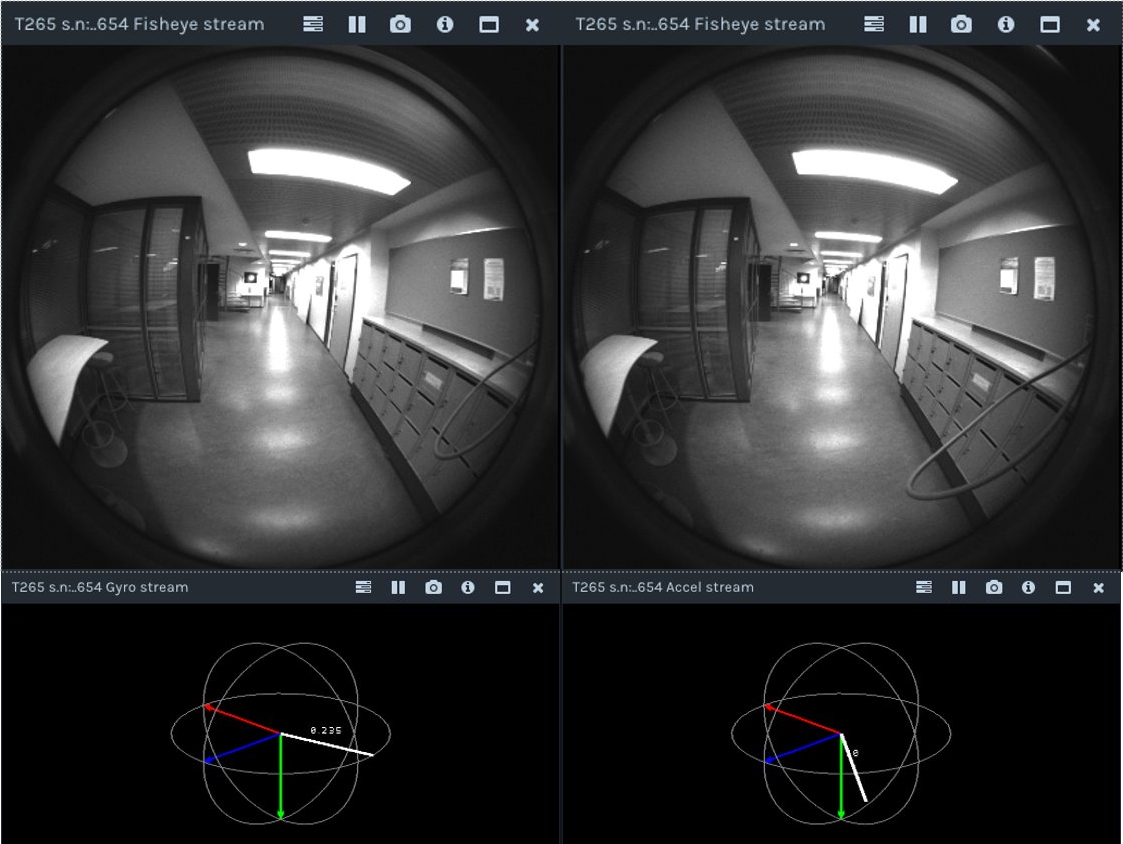
\includegraphics[height=4cm]{t265_raw.png}
        \caption{%
            Raw data from the T265.
        }\label{fig:t265_raw}
    \end{minipage}%
    \begin{minipage}[t]{.49\textwidth}
        \centering
        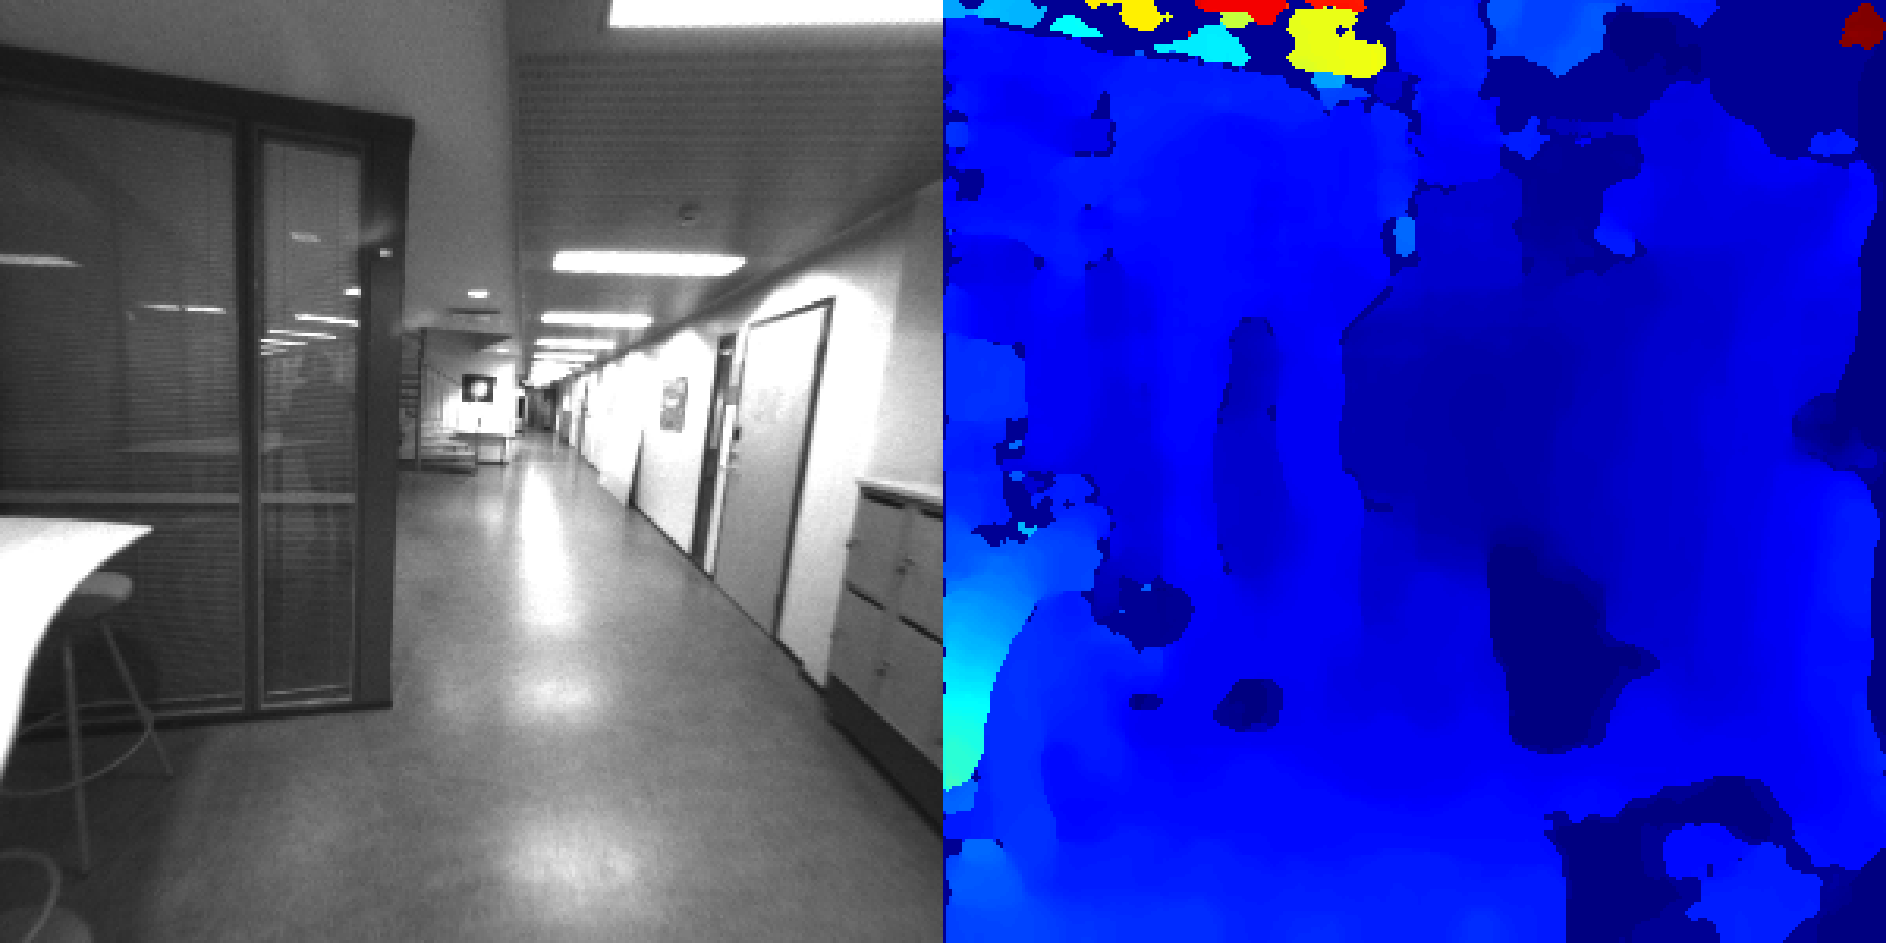
\includegraphics[height=4cm]{t265_depth.png}
        \caption{%
            Example of rectification and depth from stereo using the
            fisheye streams.
        }\label{fig:t265_depth}
    \end{minipage}%
\end{figure}

Intel RealSense is a line of computer vision sensors aimed at robotics
applications. The current generation includes the RealSense D415 and
D435\footnote{A variant with 6 \gls{dof} \gls{imu} exists as D435i.} depth
cameras and the RealSense T265 tracking camera. A lidar sensor, the RealSense
L515, is planned to hit the market in April 2020. Previous generations include
the 3D cameras F200, S200, and SR300.

The RealSense SDK (\texttt{librealsense}) is available as open source
software,\footnote{\url{https://github.com/IntelRealSense/librealsense}} and a
broad documentation is provided by
Intel\footnote{\url{https://dev.intelrealsense.com/docs/docs-get-started}},
together with a collection of code samples (available in the GitHub repository)
and tutorials. The SDK allows to seamlessly integrate multiple RealSense
devices using a uniform API.

In the lab, a RealSense D435 and a T265 are available. The D435 is a depth
camera with one RGB and two \gls{ir} global shutter sensors (87\textdegree{}
\gls{fov}), that provide RGB and rectified grayscale stereo feeds (pinhole
distortion model, 50~mm baseline). The camera performs on-board computation of a
depth map by \gls{sgm}, and it is equipped with an \gls{ir} projector that
enhances the quality of the depth, especially in textureless
areas.\footnote{Since the \gls{ir} pattern creates spurious features in the
    image, care should be put to disable it when directly using the stereo
    images in some applications (e.g.\ feature-based stereo \gls{slam}).}

The T265 is a tracking camera equipped with a 6 \gls{dof} \gls{imu} and a
stereo pair of fisheye lens sensors (163\textdegree{} \gls{fov}, 65~mm
baseline). The camera implements an on-board visual-inertial \gls{slam} system
(with loop closure and relocalisation) and provides as output the 6D pose,
together with the raw streams for the two fisheye sensors, the gyroscope and
the accelerometer (\cref{fig:t265_raw}).\footnote{The T265 is not a depth
camera, and while it is possible (on the host) to rectify the stereo images
and compute a depth map from them, the quality of such depth map is
significantly inferior to the depth camera (\cref{fig:t265_depth}). For an
example of how to rectify fisheye images and perform stereo matching,
see the example in the \texttt{librealsense} SDK:
\url{https://github.com/IntelRealSense/librealsense/blob/83f952a4bd/wrappers/python/examples/t265_stereo.py}}

The depth and tracking cameras can be combined together for 3D reconstruction
tasks. A mechanical support for both cameras is provided by Intel in the form
of a 3D
model,\footnote{\url{https://github.com/IntelRealSense/librealsense/tree/3b14a5c/examples/tracking-and-depth}}
together with a calibration
matrix,\footnote{\url{https://github.com/IntelRealSense/librealsense/blob/3b14a5c876/examples/tracking-and-depth/H_t265_d400.cfg}}
and a 3D-printed copy is already available in the lab.\footnote{Such support
    can then be mounted on a tripod, or it is possible to attach it to a
    laptop. For the latter use case, it is possible to 3D-print a fixture that
    can be taped to the lid of the laptop, and allows to attach and detach the
    camera support via its dove-tail joint. The STL file for such fixture is
available at
\url{https://github.com/m-pilia/phd-handover-report/blob/master/data/fixture.stl}.}
A calibration of the rig can be performed with Kalibr (\cref{sec:kalibr}) if
necessary.

\subsection{MyntEye}

A MyntEye S 1030 stereo camera is available in the lab. It is equipped with two
global shutter fisheye lens sensors (122\textdegree\texttimes76\textdegree,
120~mm baseline), \gls{ir} projectors, and 6 \gls{dof} \gls{imu}. The SDK is
available as open source
software\footnote{\url{https://github.com/slightech/MYNT-EYE-S-SDK}} and
includes a \gls{ros}
wrapper.\footnote{\url{https://github.com/slightech/MYNT-EYE-S-SDK/tree/master/wrappers/ros}}

The camera is not self-calibrating, and calibration of the distortion
parameters needs to be performed manually with a tool provided by the
manufacturer.\footnote{\url{https://mynt-eye-s-sdk.readthedocs.io/en/2.3.9/src/tools/calibration_tool.html}}
Camera-IMU calibration can be performed with Kalibr (\cref{sec:kalibr}).

While the higher baseline should give this camera more range, the quality of
the depth map seems worse compared to the RealSense.\footnote{The camera
available in the lab may require a new calibration of the intrinsics, including
the distortion coefficients.} The SDK and documentation are also less mature.

\subsection{ZED camera}

The ZED camera\footnote{\url{https://www.stereolabs.com/zed/}} is a stereo
camera manufactured by ZED Labs (76\textdegree\texttimes47\textdegree, 120~mm
baseline). At Tampere University, some units are available at CIVIT.

The API is fairly mature and exposes access to both raw data (streams for raw
and rectified stereo images and depth map) and high-level features (such as
mapping and 3D scanning). The SDK is however proprietary, close source
software. Another noteworthy limitation is that the depth map is computed on
the host, and the SDK requires a CUDA-enabled Nvidia GPU to work.

\subsection{OpenVSLAM}

OpenVSLAM~\cite{openvslam2019} is a \gls{slam} system developed at the National
Institute of Advanced Science and Technology in Japan. It consists of a C++
library based on OpenCV that allows to perform \gls{slam} based on pure visual
odometry, and supports multiple camera configurations as input, including
monocular, stereo, and RGB-D, with several lens models (pinhole, fisheye,
equirectangular). While being very young, the project has good quality and
coding standards, and it is currently under active development.

Detailed usage examples are
provided,\footnote{\url{https://openvslam.readthedocs.io/en/master/example.html}}
ready to run on known benchmark datasets (such as Kitti~\cite{geiger2013vision}
or TUM-VI~\cite{schubert2018vidataset}) or user data (e.g.\ on a video file). A
Docker image and a \gls{ros} package are also provided by the authors.

OpenVSLAM provides fairly good visual odometry based on point matching, by
extracting ORB~\cite{rublee2011orb} corners in each frame. It implements loop
closure detection, based on a \gls{bow} model: loop closure candidates are
searched among frames containing a sufficiently high number of corresponding
visual words and are confirmed by geometric verification. If a suitable
candidate is found, a loop closure edge is added to the pose graph, that is in
turn optimised with g2o~\cite{grisetti2011g2o}. This mechanism works reasonably
in some environments, but it easily fails in presence of perceptual aliasing
(e.g.\ when navigating through similar corridors in an office space), due to
the lack of any mechanism in the optimisation to cope with outliers produced by
the loop closure detection.

Localisation is also based on \gls{bow}, by retrieving a frame with similar
visual words and subsequently recovering the camera pose through \gls{pnp}.
This approach works on a single session \gls{slam}, but it is likely not robust
enough to handle localisation in multiple sessions with highly varying
conditions (illumination, crowding, etc.) or image data from different sensors.

While OpenVSLAM is reasonably optimised for speed, it is not optimised for
memory usage. The map can be stored to disk in messagepack format, to be
subsequently loaded in a new session, and it is kept in memory in a JSON
structure, as most other data structures in the software, therefore incurring
in a serious memory overhead. This is a limiting factor, making it impossible
to map a space significantly larger than Kampusareena when using a laptop with
32~GB of memory. Another limiting factor is the time required to perform
\gls{ba}, that grows without bounds with the size of the pose graph, requiring
several minutes to complete a loop closure on a map with a few thousand
keyframes.

\subsection{Kimera}

Kimera~\cite{rosinol2019kimera} is a software library for semantic \gls{slam}
implemented at the \gls{spark}, Massachusetts Institute of
Technology.\footnote{\url{https://github.com/MIT-SPARK/Kimera}} It is composed
of four modules:

\begin{itemize}
    \item
        Kimera-VIO,\footnote{\label{note:kimera_vio}\url{https://github.com/MIT-SPARK/Kimera-VIO}} a
        \gls{vio} library that implements the \gls{slam} frontend;
    \item
        Kimera-RPGO,\footnote{\url{https://github.com/MIT-SPARK/Kimera-RPGO}}
        a library based on GTSAM~\cite{dellaert2006square,dellaert2012factor}
        that implements pose graph optimisation for loop closures;
    \item
        Kimera-Mesher, a module that provides real-time mesh generation
        (implemented in the Kimera-VIO
        repository);\textsuperscript{\ref{note:kimera_vio}}
    \item
        Kimera-Semantics,\footnote{\url{https://github.com/MIT-SPARK/Kimera-Semantics}}
        a library that adds real-time semantic labels to the mesh.
\end{itemize}

The library can be used to implement a standalone SLAM system, and a \gls{ros}
package is provided by the
authors.\footnote{\url{https://github.com/MIT-SPARK/Kimera-VIO-ROS}}.

Kimera is a very young project and, at the time of writing, the code is not
stable. The odometry seems to be working but the loop closure integration in
the \gls{slam} system seems to be currently
broken.\footnote{\url{https://github.com/MIT-SPARK/Kimera-VIO-ROS/issues/37}}
While the code may not be practical to be directly reused, at least for the
moment, it is a noteworthy reference to previous work, especially with respect
to the integration of real-time semantics in a \gls{slam} system. It also
represents a real example of usage for GTSAM.

The pose graph optimisation in Kimera-RPGO implements robust loop closures on
top of GTSAM, with an outlier rejection mechanism~\cite{mangelson2018pairwise}.
Being separated from the rest of the system, it is possible to easily re-use it
as a building block for a different \gls{slam} solution, or use it as a
baseline for experiments on loop closure.

\subsection{\acs{rtabmap}}

\gls{rtabmap}~\cite{labbe2019rtab} is a \gls{slam} framework developed at the
\gls{introlab}, Université de Sherbrooke. It is a mature and feature-rich
framework, under active development, that provides:
\begin{itemize}
    \item visual \gls{slam} based on \gls{rgbd}, stereo, or lidar input;
    \item built-in \gls{rgbd} odometry based on point features (including
        support for SIFT~\cite{lowe1999object}, SURF~\cite{bay2006surf},
        ORB~\cite{rublee2011orb}, and other descriptors);
    \item multi-session mapping, built-in capability to import, manipulate, and
        export maps;
    \item optimisation for mapping of large environments in real-time, with
        bounded computing time per frame;
    \item built-in integration with several odometry front-ends (LOAM, FOVIS,
        Viso2, DVO, ORB\_SLAM2, OKVIS, MSCKF\_VIO, VINS-Fusion);
    \item integration with several solvers for \gls{ba} and loop closure
        (ceres~\cite{ceres-solver}, g2o~\cite{grisetti2011g2o},
        GTSAM~\cite{dellaert2006square},
        cvsba\footnote{\url{https://www.uco.es/investiga/grupos/ava/node/39}}~\cite{lourakis2009sba});
    \item integration of switchable constraints~\cite{sunderhauf2012switchable}
        for robust loop closures
        (Vertigo\footnote{\url{https://openslam-org.github.io/vertigo.html}});
    \item out-of-the-box integration with several cameras, including ZED,
        RealSense, and Kinect;
    \item runs as a standalone GUI application (Android, Linux, Mac, Windows)
        or as a \gls{ros} node;
    \item tools for debugging and introspection;
    \item a large number of options and tunable parameters;
\end{itemize}

The built-in visual odometry of \gls{rtabmap} is based on point features and
relies on depth information, accepting \gls{rgbd} or stereo input (in the
latter case, depth is computed from stereo by \gls{sgm}). The built-in odometry
is comparable to other visual \gls{slam} systems such as
ORB-SLAM2~\cite{ragot2019benchmark}.

\gls{rtabmap} produces a database file encoding the map, including keypoints,
features, and images for the keyframes, whose default location is in
\texttt{\textasciitilde/.ros/rtabmap.db}. While localisation is based on point features, it
should be relatively straightforward to use the frames collected in an
\gls{rtabmap} session to train a HF-Net~\cite{sarlin2019coarse} system in the
attempt to devise a more robust global localisation method.

Detailed documentation can be found on the GitHub
wiki\footnote{\url{https://github.com/introlab/rtabmap/wiki}} for the
standalone version and on the \gls{ros}
wiki\footnote{\url{http://wiki.ros.org/rtabmap_ros}} for the \gls{ros} package
(\texttt{rtabmap\_ros}).

Pre-built binaries for both the standalone application and for the \gls{ros}
package are available in the \gls{ros} Ubuntu repository, however the pre-built
version of the standalone application is missing several optional components
(e.g.~integration with GTSAM or RealSense). It is possible to check what
components are built in the current version by running \texttt{rtabmap
-{}-version}, and to enable more components it is necessary to build
\gls{rtabmap} from source, after installing or building the desired components
and making sure that the respective packages are detected by CMake.

Besides of the aforementioned documentation, further examples of usage are
provided on the \gls{ros}
wiki\footnote{\url{http://wiki.ros.org/rtabmap_ros/Tutorials/HandHeldMapping}}
and on the RealSense
wiki\footnote{\url{https://github.com/IntelRealSense/realsense-ros/wiki/SLAM-with-D435i}}.
The latter example shows how perform sensor fusion with an external library
(using the \texttt{robot\_localization}
package)\footnote{\url{http://wiki.ros.org/robot_localization}} to compute the
\gls{vio} externally and feed the resulting odometry to \gls{rtabmap}.

\section{Experiments}

The experiments were conducted on a Lenovo ThinkPad T480 laptop equipped with
an Intel i7--8650U CPU and 32~GB of memory. Tests were conducted both on Arch
Linux and Ubuntu 16.04. The following instructions allow to reproduce the
experimental environment on Ubuntu 16.04 or 18.04.

When reproducing the work it is recommended, even if not strictly necessary, to
install and configure \texttt{ccache}, since it can greatly speed up repeated
builds:
\begin{Verbatim}[samepage=true]
    sudo apt-get install -y ccache
    sudo /usr/sbin/update-ccache-symlinks
    echo 'export PATH="/usr/lib/ccache:$PATH"' > ~/.bashrc
    source ~/.bashrc
\end{Verbatim}

\subsection{Mapping with \acs{rtabmap}}\label{sec:rtabmap-setup}

\subsubsection{Installation}

The following instructions allow to reproduce the set-up used to test
\gls{rtabmap}:
\begin{enumerate}

    \item A clean environment on Ubuntu 16.04 (Xenial) or 18.04 (Bionic) is
        assumed. In this work, a fresh installation of Ubuntu 16.04.6 was used.

        The \texttt{realsense-ros} package is officially supported only on
        \gls{ros} kinetic on Ubuntu 16.04, but it seems to work on \gls{ros}
        melodic on Ubuntu 18.04 as well, as long as the \gls{lts} Linux kernel
        is used (version 4.15, provided by the apt package
        \texttt{linux-generic}). When replicating the results on Ubuntu 18.04,
        it is necessary to replace Xenial with Bionic and \texttt{ros-kinetic}
        with \texttt{ros-melodic} in the following instructions.

    \item Install \gls{ros} Kinetic from the \gls{ros} deb repository,
        following the upstream instruction on the
        wiki.\footnote{\url{http://wiki.ros.org/kinetic/Installation/Ubuntu}}

    \item Install the \texttt{ros-kinetic-rqt-reconfigure} package with
        \texttt{apt}. This tool is not strictly necessary, but it is useful to
        quickly inspect and change \gls{ros} parameters. Make sure that the
        tool correctly works by launching it with
\begin{Verbatim}[samepage=true]
    rosrun rqt_reconfigure rqt_reconfigure
\end{Verbatim}
        (a \texttt{roscore} instance needs to be running: if you are not sure
        what this means, a walk through the \gls{ros} tutorials is recommended
        before continuing).

    \item Install \texttt{librealsense} from the Intel deb repository,
        following the upstream instructions on
        GitHub.\footnote{\url{https://github.com/IntelRealSense/librealsense/blob/e8cb6b4/doc/distribution_linux.md\#installing-the-packages}}
        In this work, \texttt{librealsense} 1.32.0 was used.

        After the installation, connect the RealSense devices, launch
        \texttt{realsense-viewer}, and make sure that they are working
        correctly. Ensure that the depth map and the stereo images are received
        at the correct frame rate, stuttering or flickering can be symptoms of
        low level problems (e.g.\ issues with the kernel modules, or
        insufficient bandwidth on the USB controller).

    \item Install \texttt{realsense-ros}. At the time of writing, this package
        is not available as a binary distribution and needs to be built from
        source. Create a catkin workspace and build it by following the
        upstream instructions on
        GitHub.\footnote{\url{https://github.com/IntelRealSense/realsense-ros/blob/69d199d/README.md\#step-3-install-intel-realsense-ros-from-sources}}
        In this work, \texttt{realsense-ros} 2.2.12 was used.

        The workspace needs to be enabled in the shell when working with the
        cameras. The following command (from the aforementioned instructions)
        automatically enables it within any bash session:
\begin{Verbatim}[samepage=true]
    echo "source ~/catkin_ws/devel/setup.bash" >> ~/.bashrc
\end{Verbatim}
        After the installation, make sure that \texttt{realsense-ros} is
        correctly working by running one of the example launchfiles, for
        instance the point cloud publisher\footnote{\url{https://github.com/IntelRealSense/realsense-ros/blob/69d199d/README.md\#rgbd-point-cloud}}
\begin{Verbatim}[samepage=true]
    roslaunch realsense2_camera rs_camera.launch filters:=pointcloud
\end{Verbatim}
        and in another shell launch \texttt{rviz} to display the point cloud.
        In \texttt{rviz}, under the tree view displayed in the panel on the
        left dock, set the ``\texttt{Fixed frame}'' (under ``\texttt{Global
        Options}'') to \texttt{camera\_link}, and enable the point cloud by
        clicking the ``\texttt{Add}'' button on the bottom left, in the dialog
        window switch to the ``\texttt{By topic}'' tab, and select the
        \texttt{pointcloud2} topic (under
        \texttt{depth\_registered/points}).\footnote{To get familiar with
        \texttt{rviz}, a set of tutorials is available in the \gls{ros} wiki at
        \url{http://wiki.ros.org/rviz/Tutorials}.}

    \item Install \gls{rtabmap} and its \gls{ros} wrapper. The binary version
        from the \gls{ros} deb repository includes support for g2o and Vertigo,
        and was used in the experiments (with version 0.19.3)
\begin{Verbatim}[samepage=true]
    sudo apt-get install ros-kinetic-rtabmap ros-kinetic-rtabmap-ros
\end{Verbatim}

        Launch \texttt{rtabmap}, and if the installation was successful the GUI
        should open.

    \item (Optional) Some additional solvers (e.g.\ GTSAM, cvsba) and camera
        modules (e.g.\ to use RealSense devices from the standalone
        application) require to build \gls{rtabmap} from source, following
        upstream
        instructions.\footnote{\url{https://github.com/introlab/rtabmap_ros/blob/5b3fe2f/README.md\#build-from-source}}
        Before building from source, uninstall any existing \gls{rtabmap}
        binary packages from the system, to avoid unintentionally linking to
        the wrong libraries.

        When generating the build files with CMake (before
        running \texttt{make}), ensure that the desired components have been
        detected by CMake and are included in the build, by either inspecting
        the CMake console output or by opening the CMake cache and ensuring
        that the variable \texttt{WITH\_XXX} is set to \texttt{ON} (where
        \texttt{XXX} is the desired component, e.g.\ \texttt{GTSAM} or
        \texttt{CVSBA}).

\end{enumerate}

\subsubsection{Usage}

To take advantage of the high quality visual-inertial odometry provided by the
RealSense T265 tracking camera, it is possible to let \gls{rtabmap} read the
odometry directly from the T265, together with the \gls{rgbd} input from the
D435. \gls{rtabmap} performs bundle adjustment, loop closure detection, and
builds the map and point cloud. The \texttt{realsense-ros} repository already
provides a launch file named
\texttt{rs\_rtabmap.launch},\footnote{\url{https://github.com/IntelRealSense/realsense-ros/blob/69d199d9e/realsense2_camera/launch/rs_rtabmap.launch}}
located in the \texttt{realsense2\_camera} package, that allows to run
\gls{rtabmap} with this type of setup, creating a couple of \gls{ros}
nodes publishing data from each RealSense device, a node to publish the
transform between cameras, and a node that runs \gls{rtabmap} and starts
\texttt{rviz} for real-time visualisation of the point cloud being generated.
This can be started with:
\begin{Verbatim}[samepage=true]
    roslaunch realsense2_camera rs_rtabmap.launch
\end{Verbatim}

When terminating the program (e.g.\ from the console where it was launched, with
\texttt{Ctrl+C}), \gls{rtabmap} automatically saves the map to the database
located in \texttt{\textasciitilde/.ros/rtabmap.db}. By default, a clean database is created
at startup, removing any previous data present in the database. To avoid this,
and to allow incremental multi-session mapping, it is possible to remove the
flag \texttt{-{}-delete\_db\_on\_start} form the \texttt{rtabmap\_args} argument
in the \texttt{rs\_rtabmap.launch} file. When doing multi-session mapping, a
new map is created at the start of a new session, and it is merged with
the pre-existing map in the database as soon as a loop closure is established
with the previous map.

It is possible to inspect a database file using the
\texttt{rtabmap-databaseViewer} tool, that is included with the installation of
\gls{rtabmap} and allows to visualise pose graph, feature extraction, matching,
and loop closures:
\begin{Verbatim}[samepage=true]
    rtabmap-databaseViewer ~/.ros/rtabmap.db
\end{Verbatim}
The database can be also opened from within the \gls{rtabmap} GUI (``Open
database\ldots'' from the ``File'' menu), that allows then to export the point
cloud in PLY format.

Since \gls{rtabmap} is already computing loop closures, it is useful to disable
the on-board relocalisation on the T265 to avoid conflicts. This can be
achieved by setting the corresponding \gls{ros} parameter to
false\footnote{\url{https://github.com/m-pilia/realsense-ros/commit/6521e3f9738}}
\begin{Verbatim}[samepage=true]
    <rosparam>
        /t265/tracking_module/enable_relocalization: false
    </rosparam>
\end{Verbatim}
in the \texttt{rs\_rtabmap.lauch} launch file, located in
\begin{Verbatim}[samepage=true]
    "$CATKIN_WS"/src/realsense-ros/realsense2_camera/launch/rs_rtabmap.launch
\end{Verbatim}
where \texttt{\$CATKIN\_WS} is the location of the catkin workspace where the
\texttt{realsense-ros} package was built. It is possible to use
\texttt{rqt\_reconfigure} to check the value of the parameter while the system
is running (but not to change it while the camera is streaming):
\begin{Verbatim}[samepage=true]
    rosrun rqt_reconfigure rqt_reconfigure
\end{Verbatim}

\gls{rtabmap} stores its parameters in the
\texttt{\textasciitilde/.rtabmap/rtabmap.ini} configuration file. The
parameters can be modified either in the configuration file or through the
\gls{rtabmap} GUI application (taking care of saving the configuration before
leaving the GUI). In the experiments, the g2o solver was used for pose graph
optimisation, and robust loop closure detection with switchable constraints was
enabled, corresponding to the following parameters:\footnote{A copy of the
    parameter file used in the data collection is available at
\url{https://github.com/m-pilia/phd-handover-report/blob/master/data/rtabmap.ini}}
\begin{Verbatim}[samepage=true]
    Optimizer\Robust = true
    Optimizer\Strategy = 1
\end{Verbatim}
To use a custom configuration file when starting \gls{rtabmap}, it is possible
to edit the \texttt{rs\_rtabmap.launch} file and add an argument
\begin{Verbatim}[samepage=true]
    <arg name="cfg" value="/path/to/rtabmap.ini" />
\end{Verbatim}
to the \texttt{<include>} tag that includes the \texttt{rtabmap.launch} file.

In this experiment, the data was collected by fixing both cameras to the outer
surface of the laptop lid, using duct tape, and without any extrinsic
calibration. A more accurate data collection would require a rigid fix, to
prevent the two cameras from moving with respect to each other, e.g.\ by using
the 3D-printed support described in~\cref{sec:realsense}. The transformation
parameters between the two cameras can then be estimated and published using
the
\texttt{static\_transform\_publisher}\footnote{\url{http://wiki.ros.org/tf\#static_transform_publisher}}
from the \texttt{tf} package, called in the \texttt{rs\_d400\_to\_t265.launch}
file (the parameters are set to a null transform in the launch
file).\footnote{\url{https://github.com/IntelRealSense/realsense-ros/blob/69d199d9e01a/realsense2_camera/launch/rs_d400_and_t265.launch\#L48}}

\subsection{Mapping with OpenVSLAM}\label{sec:openvslam-setup}

OpenVSLAM was tested as a front-end for real-time mapping with the ZED, MYNT,
and RealSense (both D435 and T265) cameras. In order to perform SLAM in
real-time, a small prototype was implemented, with an abstract interface that
allows to use any of the four cameras. Source code and instructions are
available on
GitHub.\footnote{\url{https://github.com/m-pilia/openvslam-example}}

Note that this prototype is not production-quality code, it lacks features and
testing, and it was not designed with the idea of being published.

\subsubsection{Build}

The following instructions allow to reproduce the environment on Ubuntu 16.04
or 18.04:\footnote{The repository has a continuous integration setup,
performing cloud builds on GitHub Actions inside a Docker container. It is
possible to check the Dockerfile located in the root of the repository to
see a working example of build environment on Ubuntu.}\footnote{In the
upstream installation instructions, all software packages are installed at
system level in \texttt{/usr/local}. If preferred, it is possible to
install them in a local folder by using \texttt{make
DESTDIR=/some/local/folder install} instead of \texttt{sudo make install},
to avoid littering system paths with files outside of the package manager's
control. When doing so, it is important to point CMake to such custom
installation path when each package is required in a subsequent build, by
adding an argument to CMake in the form
\texttt{-DPackageName\_DIR=/some/local/folder/path/to/config}, where
\texttt{PackageName} is the name of the CMake package and the given path
points to the CMake configuration file for the software package (e.g.
\texttt{-DOpenCV\_DIR=/home/foo/dev/share/OpenCV} if OpenCV was installed
with \texttt{make DESTDIR=/home/foo/dev install}). For more details, please
refer to the documentation of CMake:
\url{https://cmake.org/cmake/help/latest/manual/cmake-packages.7.html}.}\footnote{These
instructions assume a clean system. It would be wise to not have any \gls{ros}
or catkin workspace active in a shell used to build non-ROS software, to
prevent CMake from unexpectedly picking different versions of libraries from
ROS packages, potentially causing build or link time errors.}

\begin{enumerate}
    \item (Only on Ubuntu 16.04) Install an up-to-date version of CMake with
        support for C++17 (the default version 3.1 shipped with Ubuntu 16.04
        does not provide it).
\begin{Verbatim}[samepage=true]
    wget -O - https://apt.kitware.com/keys/kitware-archive-latest.asc 2>/dev/null \
        | sudo apt-key add -
    sudo apt-add-repository 'deb https://apt.kitware.com/ubuntu/ xenial main'
    sudo apt-get update
    sudo apt-get install -y cmake
\end{Verbatim}

    \item (Only on Ubuntu 16.04) Install a more recent version of gcc, since
        the one shipped with Ubuntu 16.04 (gcc 5.4) does not have full support
        for C++17.
\begin{Verbatim}[samepage=true]
    sudo add-apt-repository ppa:ubuntu-toolchain-r/test
    sudo apt-get update
    sudo apt-get install -y gcc-7 g++-7
    [ ! -f /usr/sbin/update-ccache-symlinks ] || sudo /usr/sbin/update-ccache-symlinks
\end{Verbatim}

    \item Build and install the OpenVSLAM library and its dependencies,
        following upstream
        instructions.\footnote{\url{https://openvslam.readthedocs.io/en/master/installation.html}}
        When building OpenVSLAM, add \texttt{-DINSTALL\_PANGOLIN\_VIEWER=ON} to
        the parameters passed to CMake when generating the build
        configuration.\footnote{The complete CMake command for this build can
        be seen at
        \url{https://github.com/m-pilia/openvslam-example/blob/8f0157575a8/Dockerfile\#L78-L87}}\footnote{In
        case multiple versions of Eigen or OpenCV were present on the system
        and the wrong one was selected in the build configuration, it is
        possible to point CMake to the correct versions by adding
        \texttt{-DEigen3\_DIR=/usr/local/share/eigen3/cmake} and
        \texttt{-DOpenCV\_DIR=/usr/local/share/OpenCV} to the CMake flags.}

        After building OpenVSLAM, install it by running \texttt{sudo make
        install} in the OpenVSLAM build folder. In these tests, OpenVSLAM up to
        commit \texttt{f2945209fc} was used.

    \item Install \texttt{librealsense} as described in
        \cref{sec:rtabmap-setup}.

    \item Install the
        MYNT-EYE-S-SDK.\footnote{\url{https://github.com/slightech/MYNT-EYE-S-SDK}}
        The SDK is available both as pre-built deb package or source
        distribution. It is recommended to build it from source after
        installing OpenCV, in order to use the same version of the library and
        avoid binary conflicts due to different versions of OpenCV, following
        upstream
        instructions.\footnote{\url{https://mynt-eye-s-sdk.readthedocs.io/en/latest/src/sdk/install_ubuntu_src.html}}

    \item (Optional) Install the ZED SDK following upstream
        instructions.\footnote{\url{https://www.stereolabs.com/developers/release/}}
        This is only required in order to use the ZED camera, and requires a
        CUDA-enabled Nvidia GPU on the host.

    \item Build the \texttt{openvslam-example} application. By default, the
        package is built with support for RealSense and MYNT. It is possible to
        optionally build it with support for the ZED camera. The ZED module is
        however untested in its current state, after refactoring and port to
        the version 3.0 of the ZED SDK, because the camera was not available
        lately, therefore it may not work as intended.
\begin{Verbatim}[samepage=true]
    git clone https://github.com/m-pilia/openvslam-example
    cd openvslam-example
    mkdir build && cd build

    # Only on Ubuntu 16.04, use gcc-7 instead of gcc-5
    # Change to /usr/bin/{gcc,g++}-7 if not using ccache
    export CC=/usr/lib/ccache/gcc-7
    export CXX=/usr/lib/ccache/g++-7

    cmake .. # To build ZED support, use: cmake .. -DCAMERA_SLAM_WITH_ZED=ON
    make -j"$(nproc)"
\end{Verbatim}

\end{enumerate}

\subsubsection{Usage}

The build procedure will produce a \texttt{camera\_slam} executable. To see the
available parameters:
\begin{Verbatim}[samepage=true]
    ./camera_slam --help
\end{Verbatim}

Running a \gls{slam} mapping session requires to provide a destination for the
output map file, an ORB vocabulary,\footnote{A pre-built vocabulary can be
downloaded from the OpenVSLAM project at
\url{https://openvslam.readthedocs.io/en/master/simple_tutorial.html}.} and a
configuration file. Example configuration files are provided in the
\texttt{param} folder in the repository.

\begin{Verbatim}[samepage=true]
    ./camera_slam \
        -m RealSense \
        -c ../param/realsense_stereo.yaml \
        -v ../third_party/vocab/orb_vocab.dbow2 \
        --output-map-db map.msg
\end{Verbatim}

If everything works correctly, a couple of windows should open, showing the
pose graph and the current frame respectively (\cref{fig:openvslam_mapping}).

\begin{figure}[tb]
    \centering
    \begin{subfigure}[t]{.59\textwidth}
        \centering
        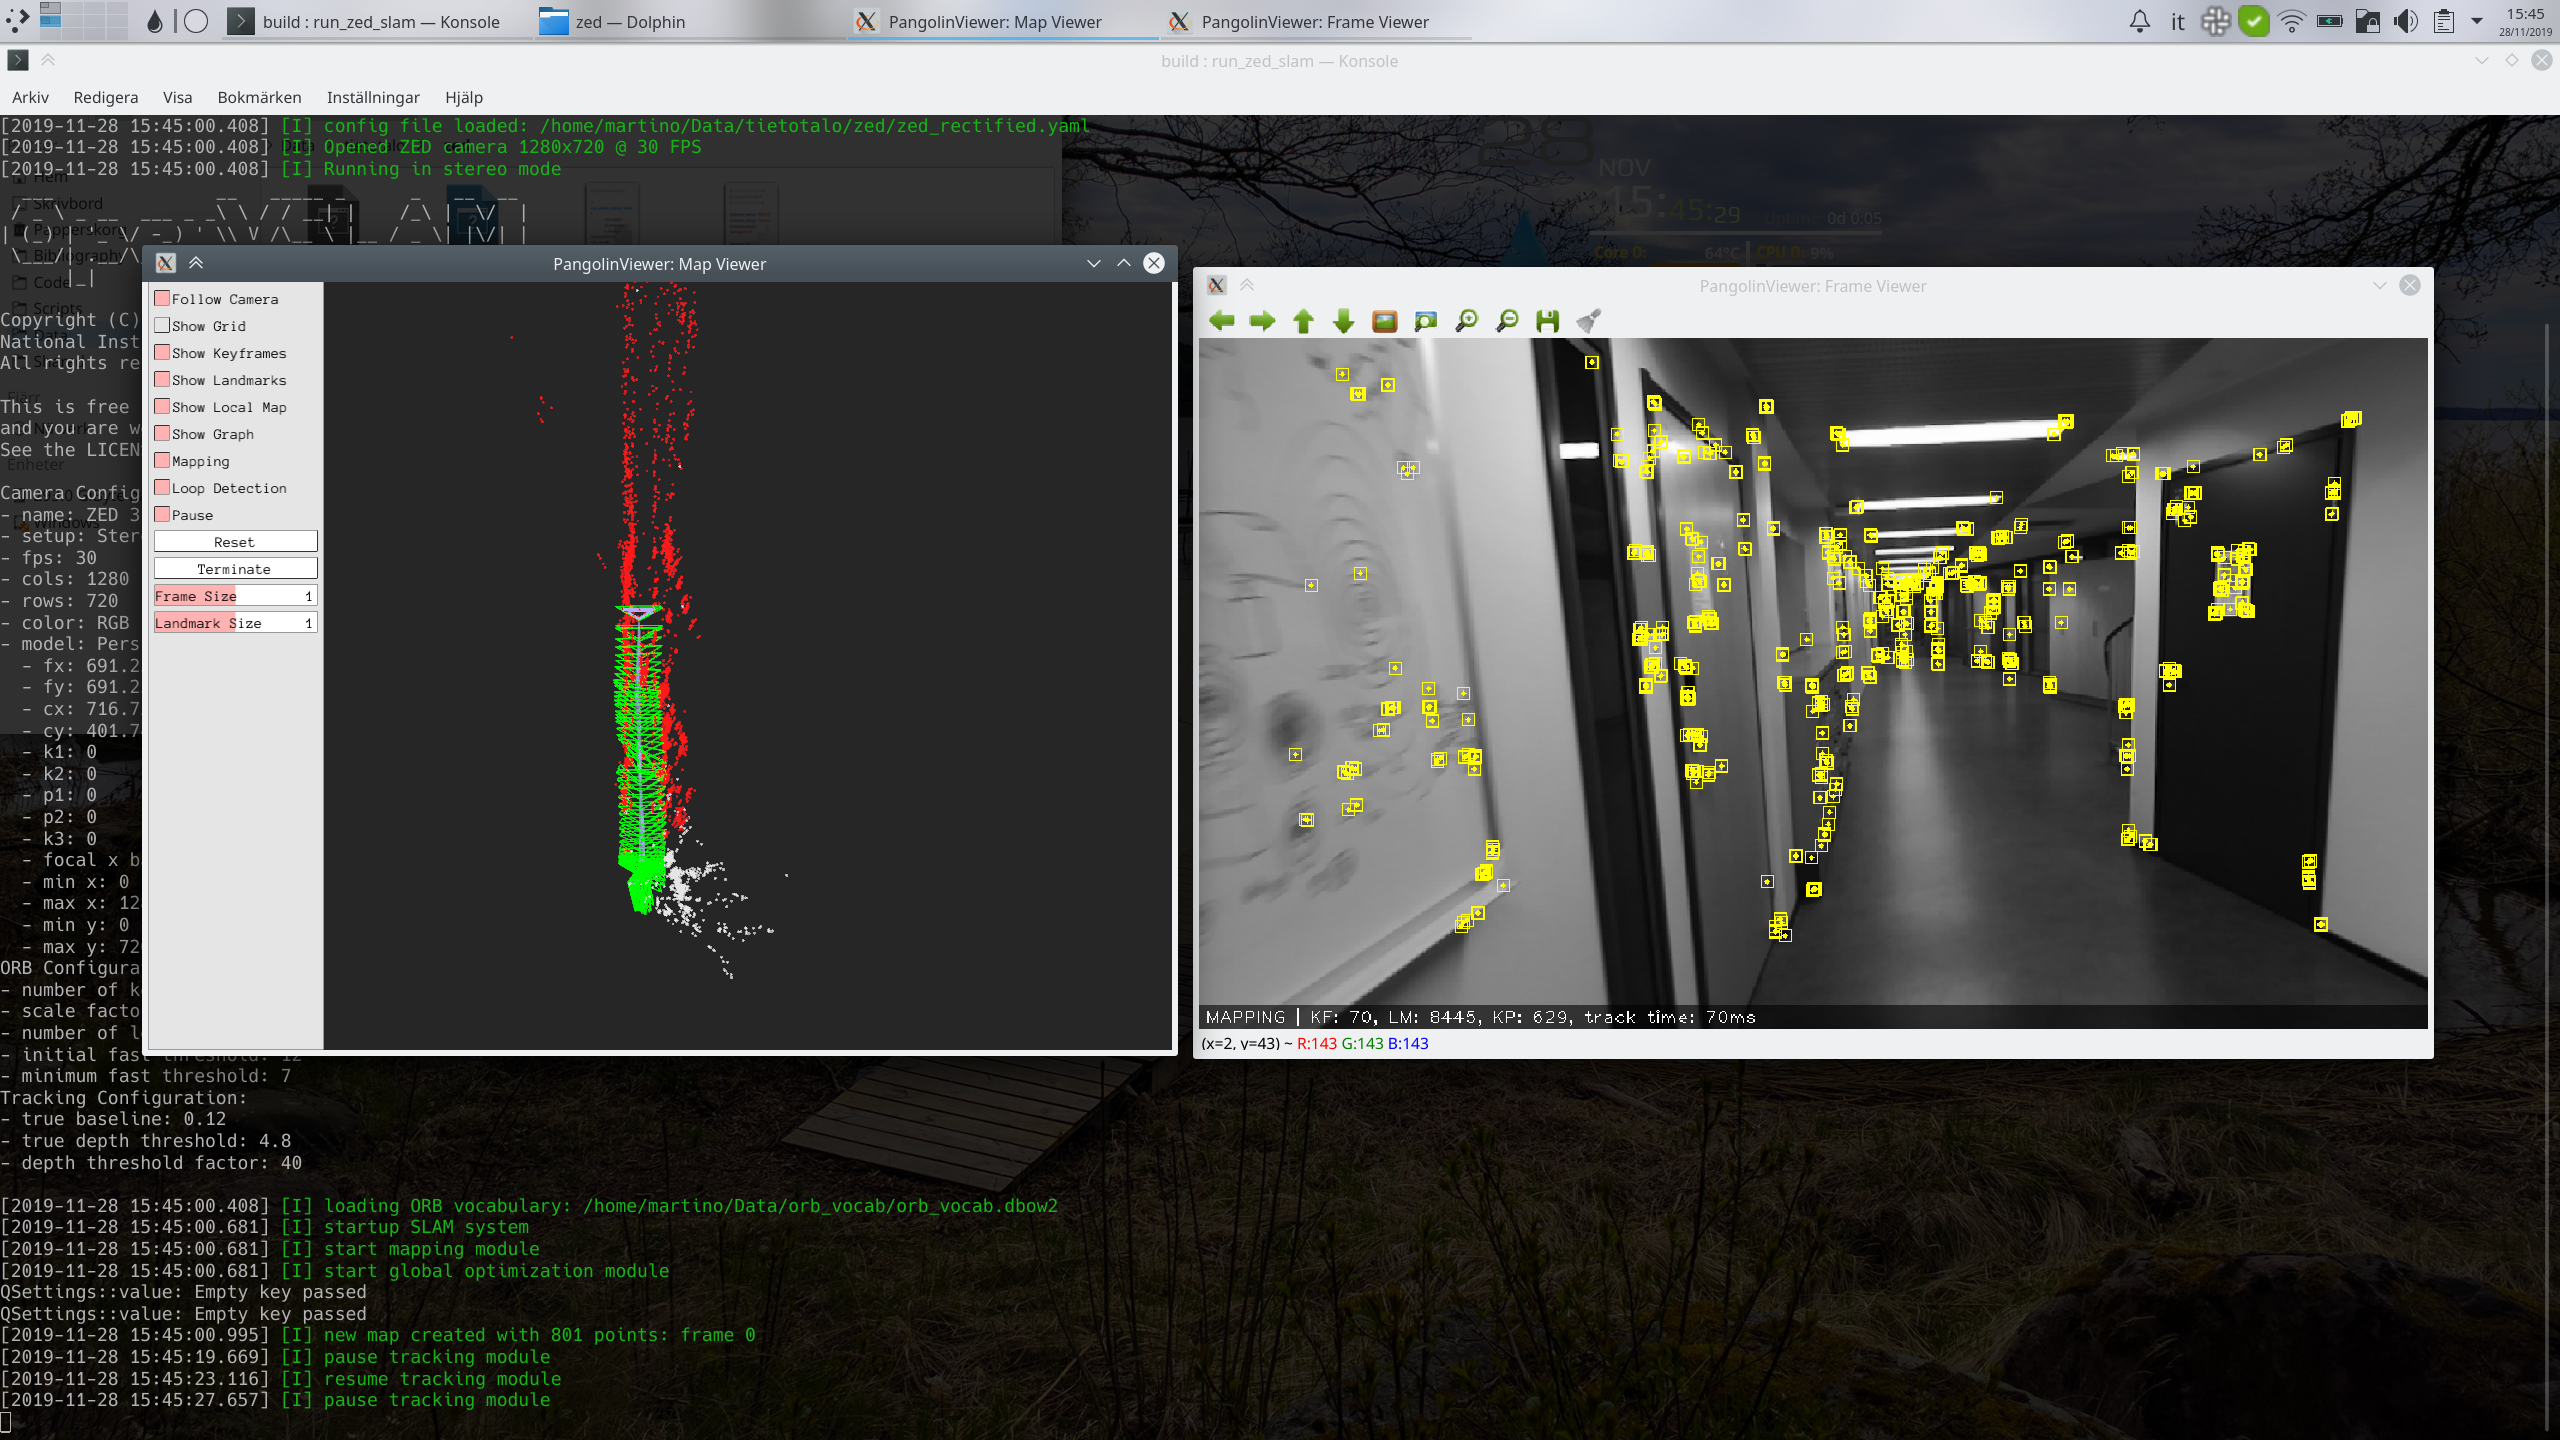
\includegraphics[height=5cm]{openvslam.png}
        \caption{Example mapping session.}\label{fig:openvslam_mapping}
    \end{subfigure}
    \begin{subfigure}[t]{.39\textwidth}
        \centering
        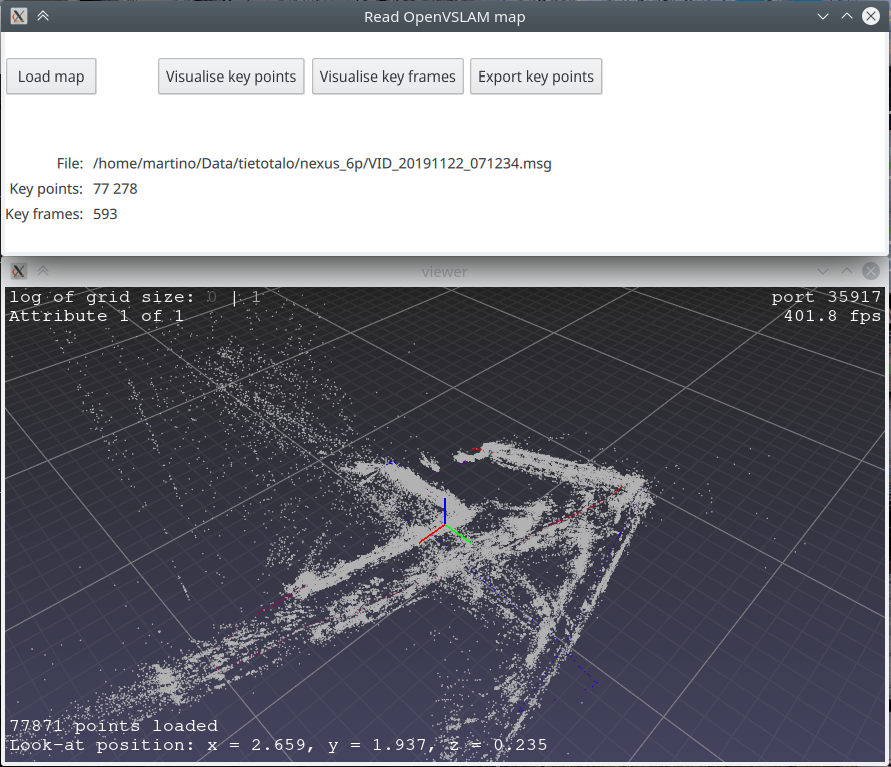
\includegraphics[height=5cm]{load_map.png}
        \caption{Example point cloud visualisation.}\label{fig:openvslam_load_map}
    \end{subfigure}
    \caption{Example of OpenVSLAM usage.}\label{fig:openvslam}
\end{figure}

To run a pure localisation session, it is necessary to load a pre-built map:

\begin{Verbatim}[samepage=true]
    ./camera_slam \
        --localization \
        -m RealSense \
        -c ../param/realsense_stereo.yaml \
        -v ../third_party/vocab/orb_vocab.dbow2 \
        --input-map-db map.msg
\end{Verbatim}

The \texttt{-{}-output-video} and \texttt{-{}-input-video} flags allow to
record and playback input data from file respectively. The output format
depends on the camera used (SVO for the ZED camera, \gls{ros} bagfile for the
RealSense, and a custom binary dump for the MYNT EYE\footnote{At the time of
writing, the MYNT EYE does not provide a raw data record and playback API,
so a very simplified mechanism was implemented in this repository.}).

The map is stored by OpenVSLAM as a messagepack dump (i.e.\ binary compressed
JSON), storing 3D keypoints with descriptors and keyframes with pose graph. A
simple Python tool is provided in the repository in order to inspect the map
(\cref{fig:openvslam_load_map}).

\begin{Verbatim}[samepage=true]
    # Install dependencies (example on Ubuntu 16.04)
    apt-get update -y
    apt-get install -y --no-install-recommends python3 python3-pip \
        python3-pyqt5 python3-pyqt5.qtopengl python3-pyqt5.qtquick \
        python3-setuptools python3-venv qml-module-* qmlscene

    # Setup virtual environment
    python3 -m venv ./scripts/.venv
    source ./scripts/.venv/bin/activate
    pip install -r ./scripts/requirements.txt

    # run the tool
    python ./scripts/read_map.py
\end{Verbatim}

Note that OpenVSLAM does not produce a dense 3D reconstruction, so additional
work is required to build a dense RGB point cloud on top of the map.

\subsection{Kimera-VIO}\label{sec:kimera-setup}

Kimera-VIO was tested using the \gls{ros} wrapper provided by the authors, simply
adding a launch file and configuration for the MyntEye~S~1030 camera.

A working \gls{ros} environment is required. In this work, \gls{ros} Kinetic
was used, and the \gls{ros} environment should be already set up if the steps
described in~\cref{sec:rtabmap-setup} were followed. To test Kimera:

\begin{enumerate}
    \item Install the MYNT-EYE-S-SDK as described in \cref{sec:openvslam-setup}.

    \item Install the MYNT-EYE-S-SDK \gls{ros} wrapper, following upstream
        instructions.\footnote{\url{https://github.com/slightech/MYNT-EYE-S-SDK/tree/master/wrappers/ros}}
\end{enumerate}

Launch and configuration files for the MYNT EYE S camera are available on a
fork of the Kimera-VIO-ROS repository, branch
\texttt{mynt-eye-s}.\footnote{\url{https://github.com/m-pilia/Kimera-VIO-ROS/tree/mynt-eye-s}}

\begin{Verbatim}[samepage=true]
    git clone https://github.com/m-pilia/Kimera-VIO-ROS
    cd Kimera-VIO-ROS
    git checkout mynt-eye-s
\end{Verbatim}

To reproduce the results, do not follow upstream build instructions, but rather
the instructions provided in the \texttt{README.md} file in the aforementioned
branch,\footnote{\url{https://github.com/m-pilia/Kimera-VIO-ROS/blob/mynt-eye-s/README.md}}
since they contain some corrections to address issues with the build.

To launch the Kimera SLAM system, after building the \gls{ros} package, start
the MYNT EYE wrapper and then use the \texttt{kimera\_ros\_mymynt.launch} file
(provided in the same \texttt{mynt-eye-s} branch):
\begin{Verbatim}[samepage=true]
    roslaunch mynt_eye_ros_wrapper display.launch
    roslaunch kimera_vio_ros kimera_ros_mymynt.launch
\end{Verbatim}

\section{Results}

\subsection{\acs{rtabmap}}

\gls{rtabmap} was tested in indoor environments. A mapping session was
conducted walking for about 2.4~km through four buildings of the Hervanta
campus, Tampere University (\cref{fig:campus_map}). First and second floor of
Kampusareena were mapped, together with the two lower floors of the main
building, the first floor of Rakennustalo, and part of the first floor of
Sähkötalo. The mapping session took about one hour and produced 1.2 million
keypoints and a pose graph containing about 3~300 nodes, with a resulting
database of size equal to 1.3~GB. The result is shown
in~\cref{fig:rtabmap_hervanta,fig:rtabmap_hervanta_detail}.

\gls{rtabmap} was able to handle the large environment and all loop closures,
despite of very long loops, with no false positives. The program required a
relatively modest amount of resources, using only about 4~GB of memory.

This experiment was meant to demonstrate the applicability of \gls{rtabmap}
rather than to generate an optimal point cloud, and it was performed in
sub-optimal conditions due to the crowded environment, that caused the presence
of bystanders and moving passer-bys in the point cloud. Moreover, the scanning
intentionally did not cover all surfaces encountered in the environments, in
order to save time, therefore the point cloud is incomplete and has holes in
it.

The importance of using a robust loop closure method is shown in a smaller
experiment, mapping a corridor in an office space in the third floor of the
Tietotalo building, where wrong loop closures are established due to perceptual
aliasing in repetitive environments~\cite{lajoie2019modeling}, if switchable
constraints~\cite{sunderhauf2012switchable} are not used in the pose graph
optimisation (\cref{fig:rtabmap_lc}).

\begin{figure}[tb]
    \centering
    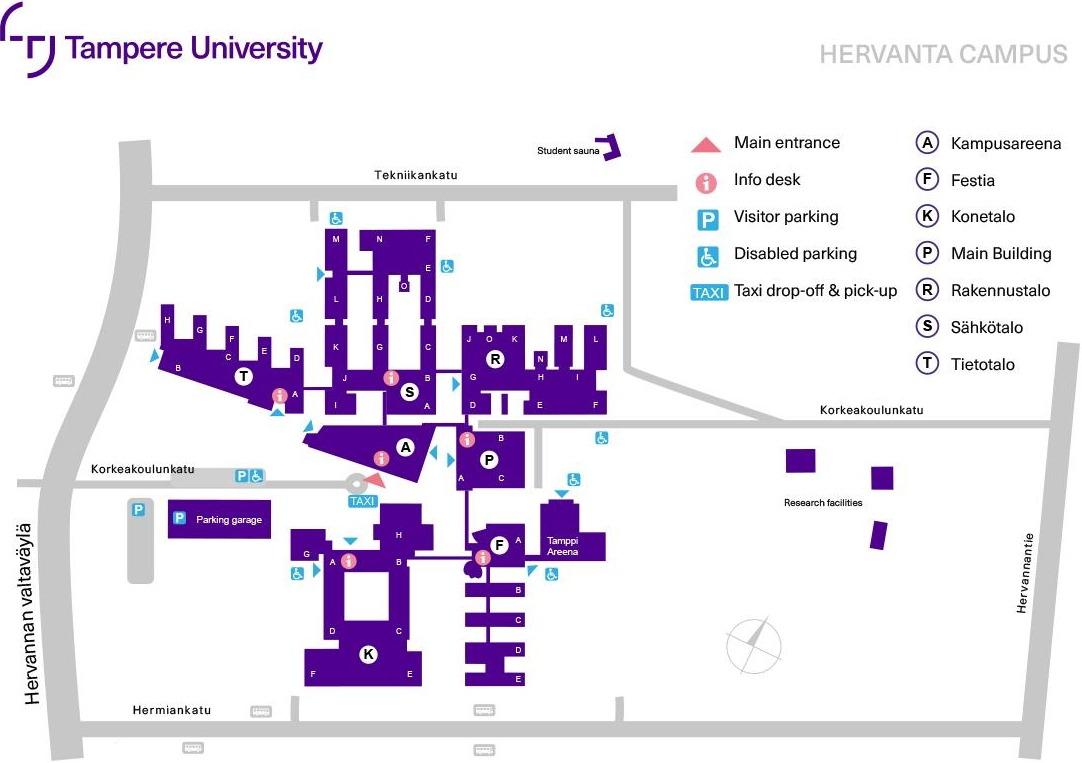
\includegraphics[width=0.9\linewidth]{campus_map.jpg}
    \caption{Map of Hervanta Campus, Tampere University.}\label{fig:campus_map}
\end{figure}

\begin{figure}[tb]
    \centering

    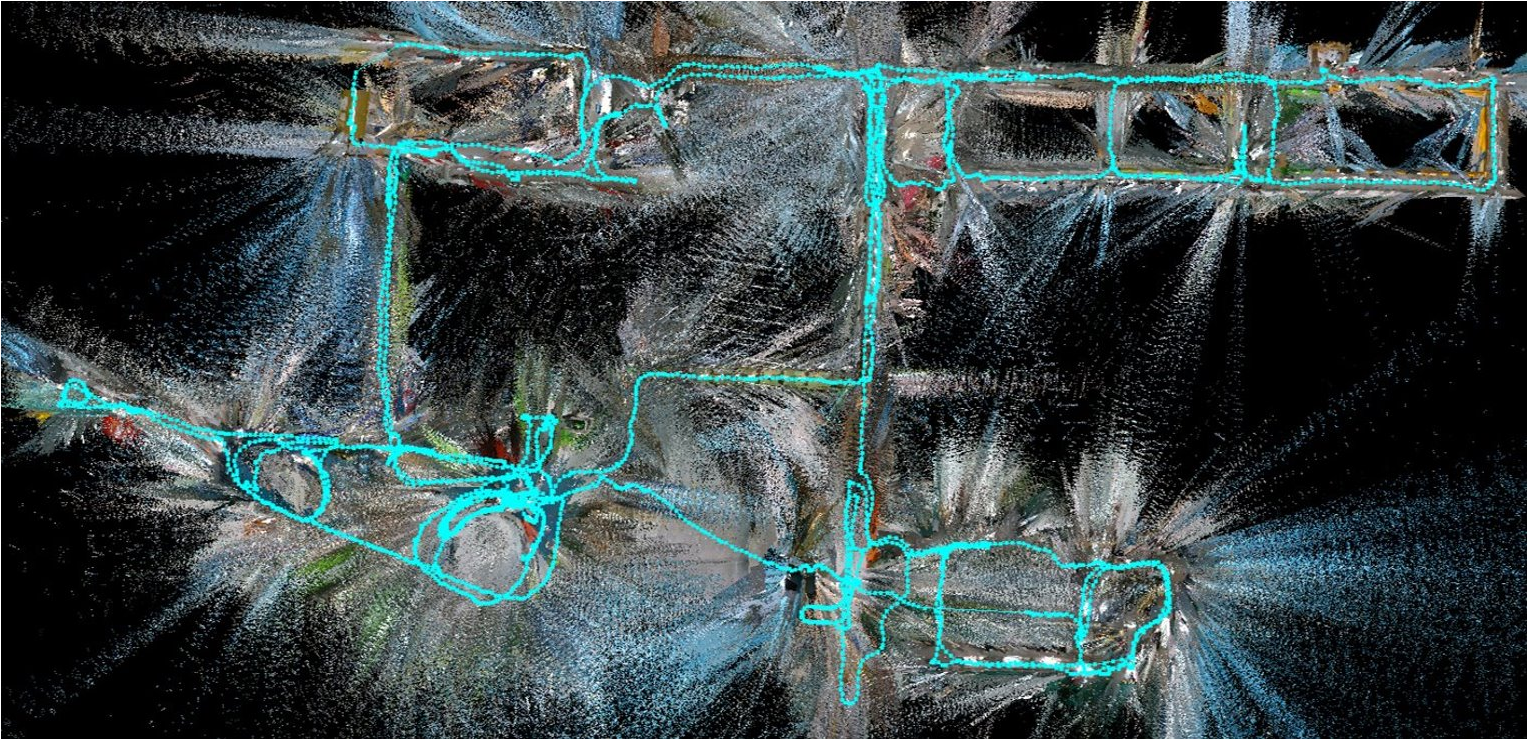
\includegraphics[width=\textwidth]{rtabmap_hervanta.png}
    \caption{%
        Point cloud of four buildings in Hervanta Campus
        (\cref{fig:campus_map}), generated with \gls{rtabmap}.
    }\label{fig:rtabmap_hervanta}

    \vspace{1em}

    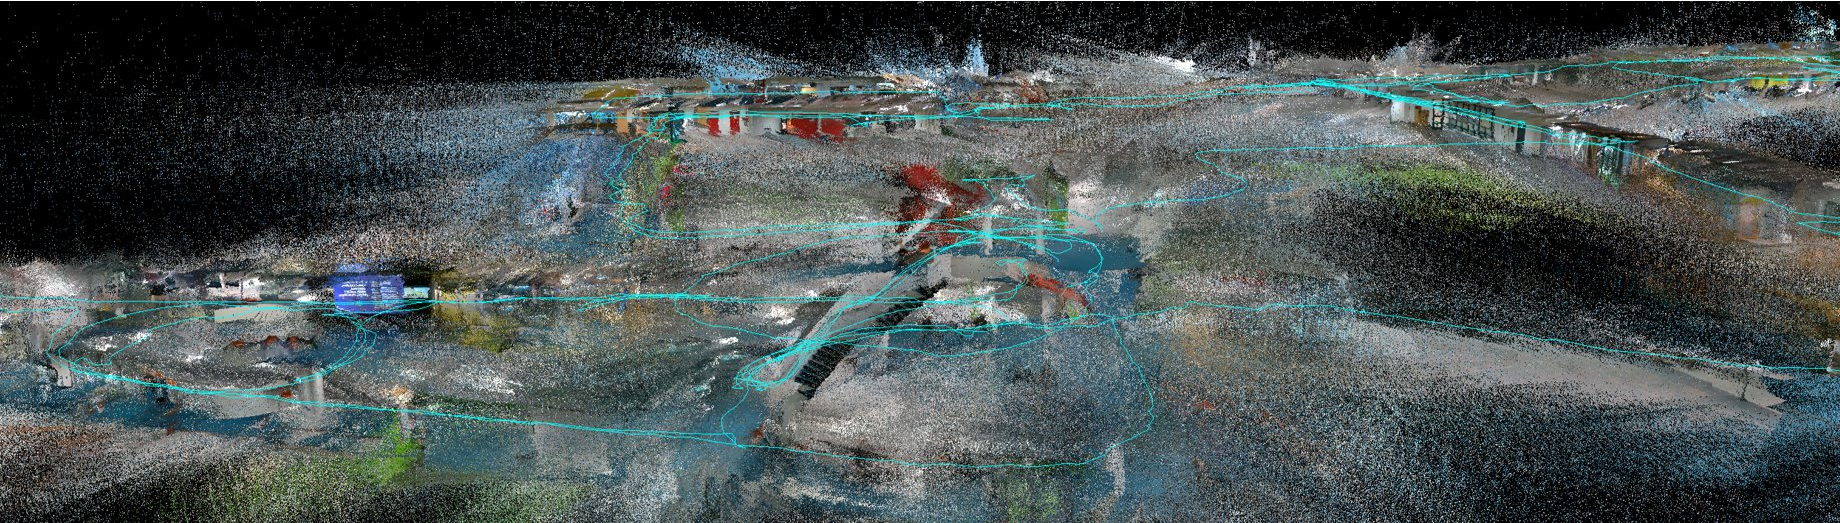
\includegraphics[width=\textwidth]{rtabmap_hervanta_detail.png}
    \caption{%
        Detail of Kampusareena from the point cloud in~\cref{fig:rtabmap_hervanta}.
    }\label{fig:rtabmap_hervanta_detail}

    \vspace{1em}

    \begin{subfigure}[t]{.34\textwidth}
        \centering
        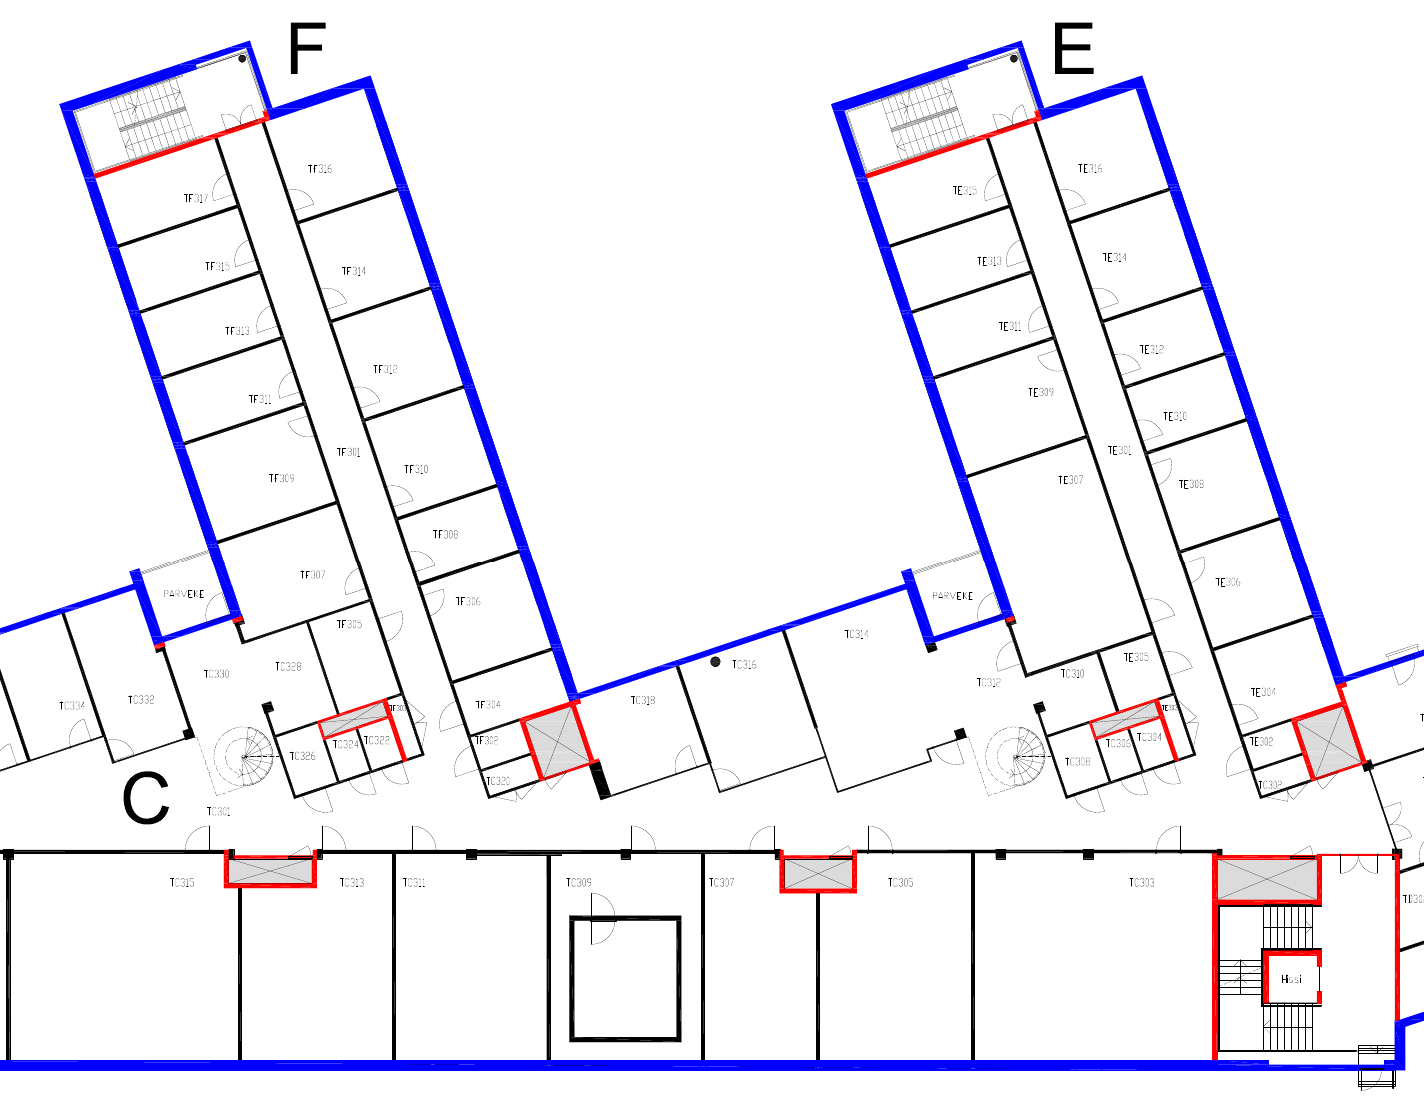
\includegraphics[height=4cm]{corridor}
        \caption{Floor plan.}\label{fig:rtabmap_lc_floorplan}
    \end{subfigure}%
    \begin{subfigure}[t]{.19\textwidth}
        \centering
        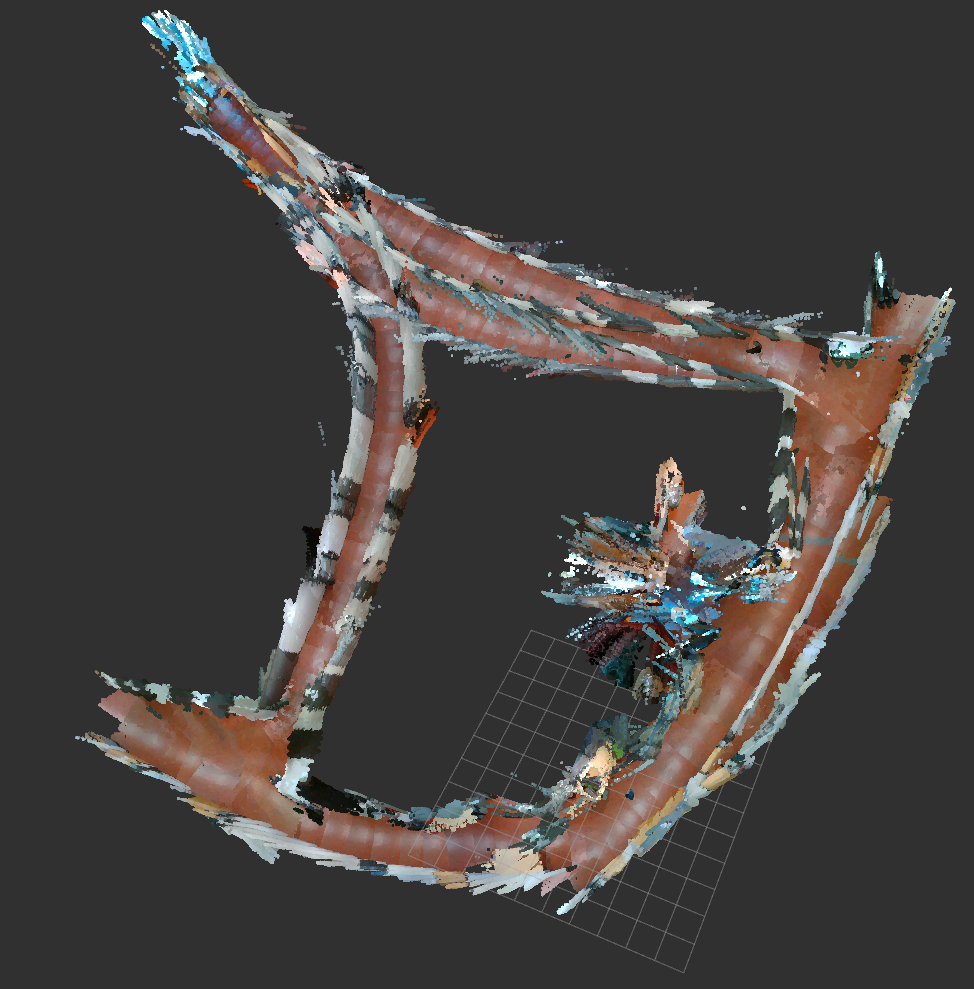
\includegraphics[height=4cm]{rtabmap_without_sc.png}
        \caption{Map without SC.}\label{fig:rtabmap_lc_without_sc}
    \end{subfigure}%
    \begin{subfigure}[t]{.44\textwidth}
        \centering
        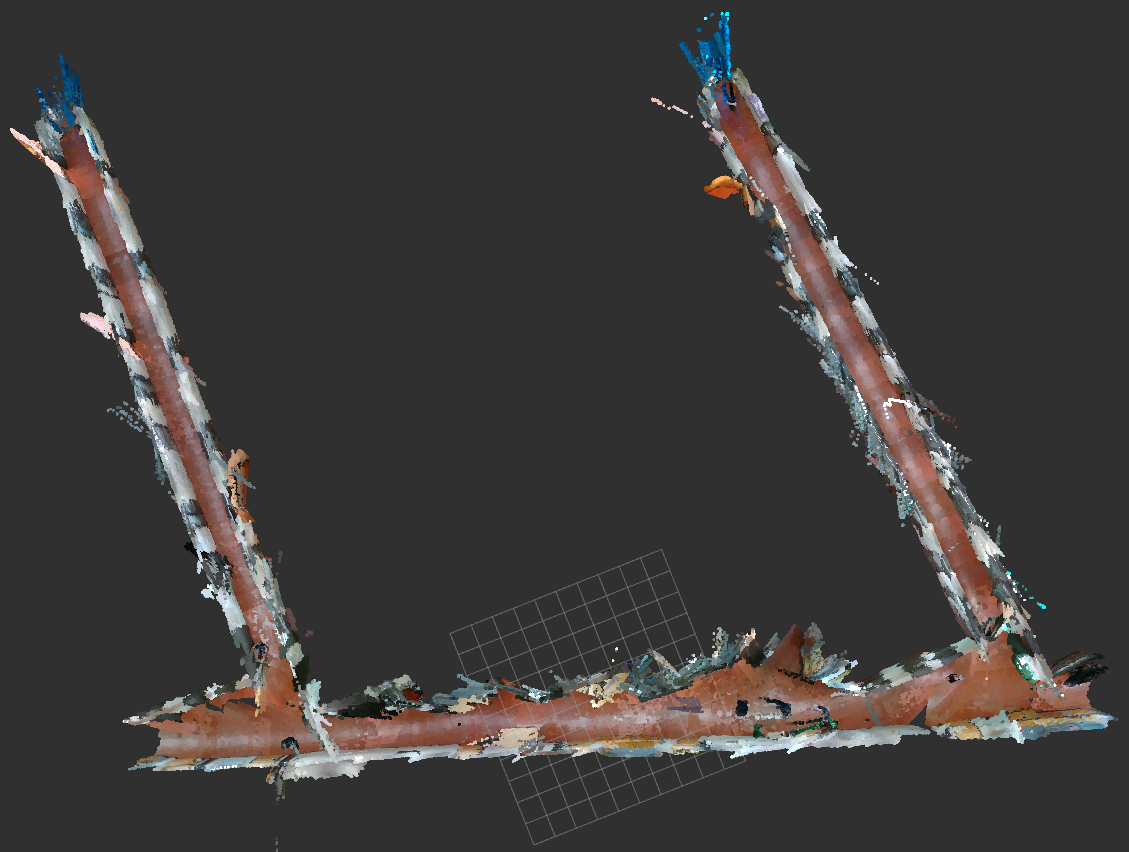
\includegraphics[height=4cm]{rtabmap_with_sc.png}
        \caption{Map with SC.}\label{fig:rtabmap_lc_with_sc}
    \end{subfigure}

    \caption{%
        Effect of switchable constraints on loop closure detection when
        scanning a corridor in an office space with \gls{rtabmap}. The g2o
        solver was used for pose graph optimisation.
    }\label{fig:rtabmap_lc}
\end{figure}

\subsection{OpenVSLAM}

\subsubsection{Mapping in presence of visual aliasing}

Since OpenVSLAM does not implement any mechanism to cope with outliers in loop
closure detection, one limitation is that it can introduce wrong loop closures
in presence of visual aliasing. An experiment was conducted by mapping the
corridor of an office space in the third floor of Tietotalo, Hervanta Campus
(\cref{fig:campus_map}), using as input the rectified stereo pair from the ZED
camera.

Results are shown in \cref{fig:openvslam_lc}. When loop closure detection was
enabled, wrong loop closures were established between similar looking
corridors. When disabling loop closures, drift was observed in the resulting
map.

\subsubsection{Mapping in large indoor environments}

An experiment was conducted by mapping first and second floor of Kampusareena
and the corridor going from Kampusareena to the third floor of Tietotalo, using
as input the rectified stereo pair from the ZED camera. The resulting map,
composed of 223~725 keypoints, is shown in
\cref{fig:openvslam_kampusareena_top,fig:openvslam_kampusareena_side}.

It is possible to observe some drift, for instance between the two floors of
Kampusareena in the circular balconies. A certain amount of drift was also
observed in the stairwell of Tietotalo, in the long corridor in Sähkötalo, and
in the bridge between Sähkötalo and Kampusareena. This could have however been
reduced by collecting data in a way that would allow more frequent loop
closures.

\subsubsection{Mapping and localisation in Kampusareena}

Another experiment was conducted to generate a more accurate map of the first
and second floor of Kampusareena, also using input from the ZED camera. The
data was collected early in the morning, with no passer-bys or people in the
scene. The cloud of keypoints is shown in
\cref{fig:openvslam_kampusareena_map_top,fig:openvslam_kampusareena_map_side}.
The map consists of 396~723 keypoints and was generated with about 2 hours of
data collection. Memory usage increased with the size of the map, peaking at
over 20~GB. Moreover, the computing time required to perform bundle adjustment
for loop closures grew with the size of the map, taking several minutes to
perform a loop closure toward the end of the mapping session.

A video demonstration of localisation in this map is available at
\url{https://github.com/m-pilia/phd-handover-report/blob/master/data/localisation_stereo.mp4}.
The video contains a sequence of short clips, and for each clip global
localisation was attempted. The video was not edited and the clips are shown in
their entirety, the jumps are due to the fact that the clips were collected in
a non-contiguous manner. These data were collected with the same camera used in
the mapping, but at a different time of the day, with more crowded environment,
and shops open, with lights on and shutters raised up or doors open.

As it is possible to observe, localisation can be very fast or sometimes take
longer, and in some parts of the map it seems to fail almost completely,
possibly due to the differences in visual appearance of the environment between
mapping and localisation. This may be due to the fact that many keypoints are
placed on non-fixed objects such as chairs, tables, posters, doors, roller
shutters of shops, etc.

\subsection{Kimera}

An experiment was conducted to map a corridor in the third floor of Tietotalo
with Kimera-VIO, using the \gls{ros} wrapper provided by the authors, with
visual-inertial input from the MyntEye~S~1030 camera. The resulting map is
shown in \cref{fig:kimera}.

The software had an increasing delay in the processing, possibly due to frame
processing being too slow with respect to the frame rate of the camera. It was
not possible to test loop closures, because enabling them would cause the
software to
crash.\footnote{\url{https://github.com/MIT-SPARK/Kimera-VIO-ROS/issues/37}}

\begin{figure}[tb]
    \centering

    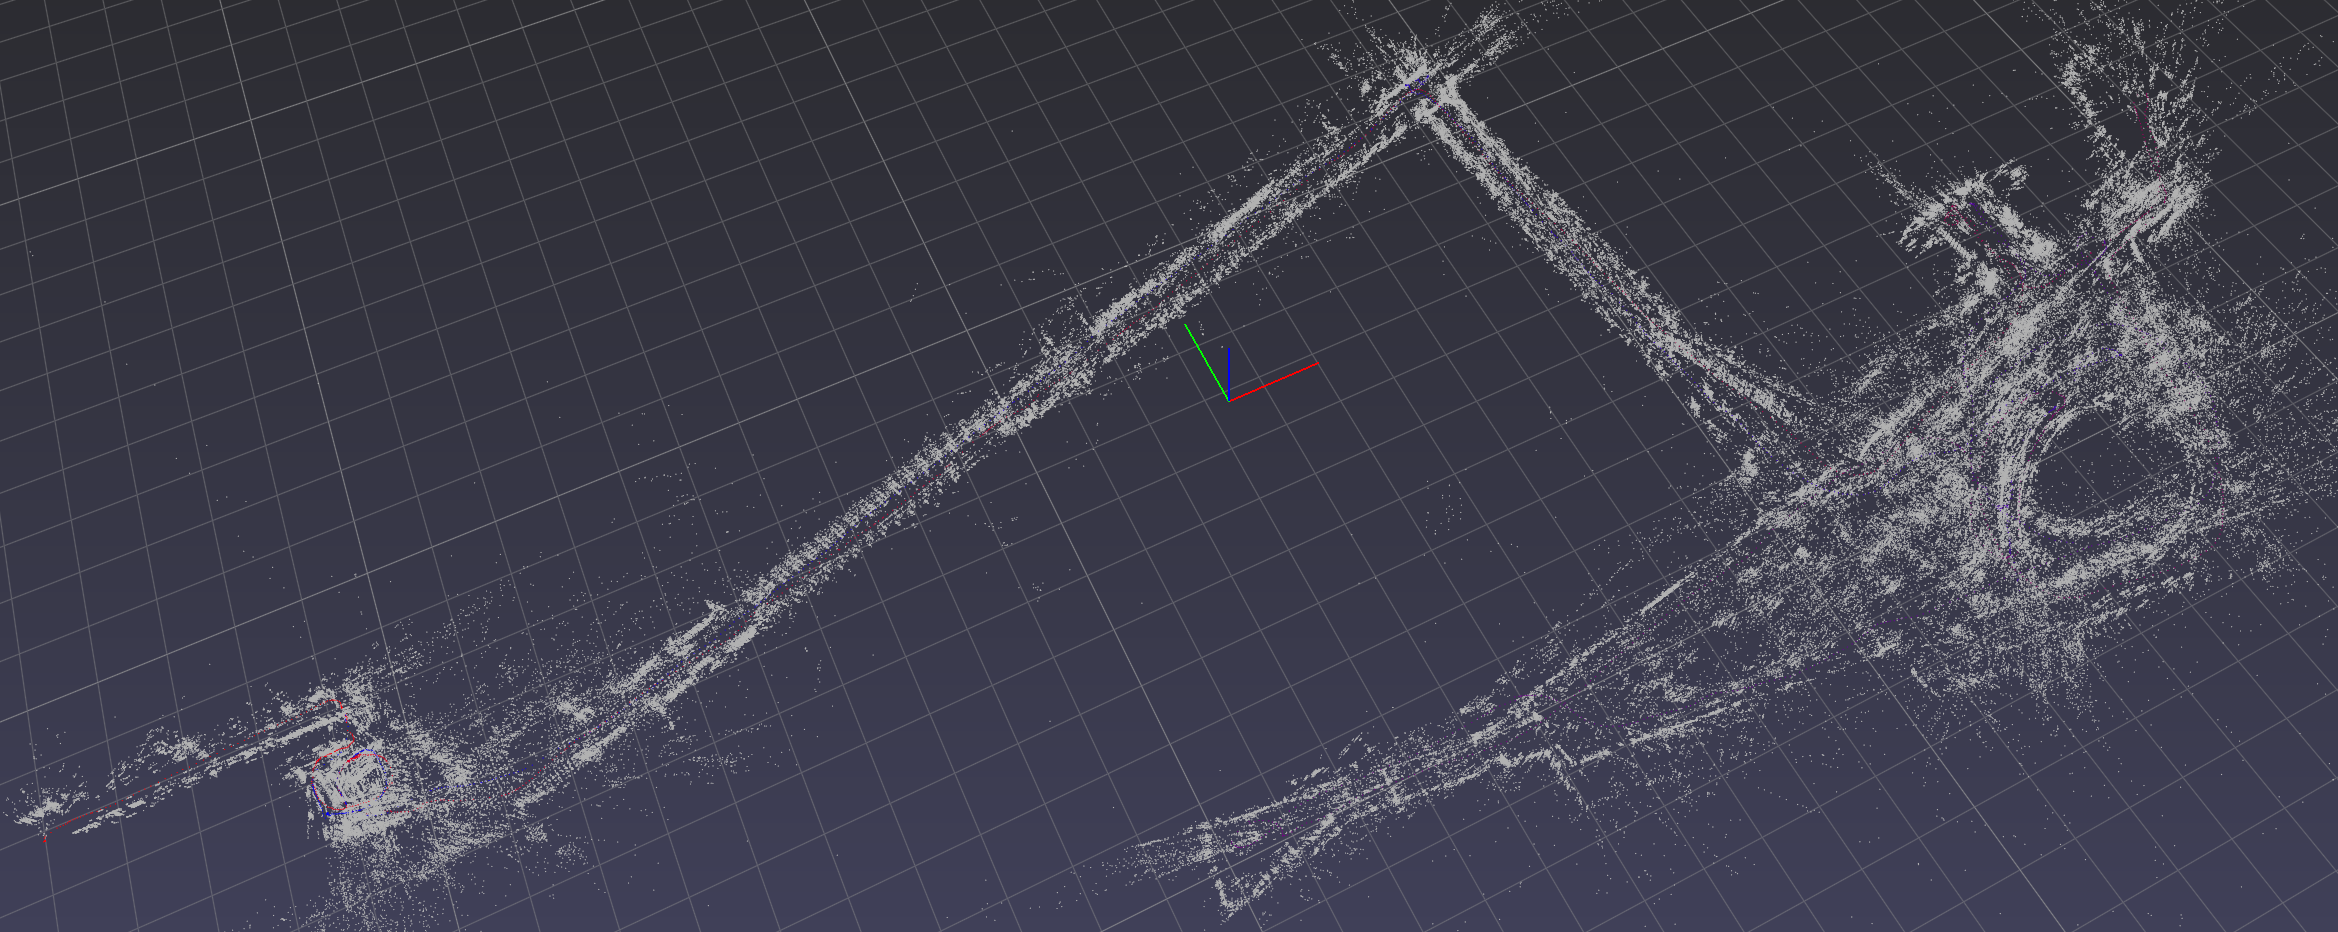
\includegraphics[width=\textwidth]{openvslam_kampusareena_top.png}
    \caption{%
        Mapping of the first and second floor of Kampusareena and the corridor
        up to the third floor of Tietotalo (223~725 points), generated with
        OpenVSLAM using as input the rectified stereo pair from the ZED camera.
        Some drift is noticeable between the two floors of Kampusareena, in the
        circular balconies. Drift is also noticeable in the long corridor and
        in the bridge between Sähkötalo and Kampusareena, but additional loop
        closures could have helped reducing it.
    }\label{fig:openvslam_kampusareena_top}

    \vspace{1em}

    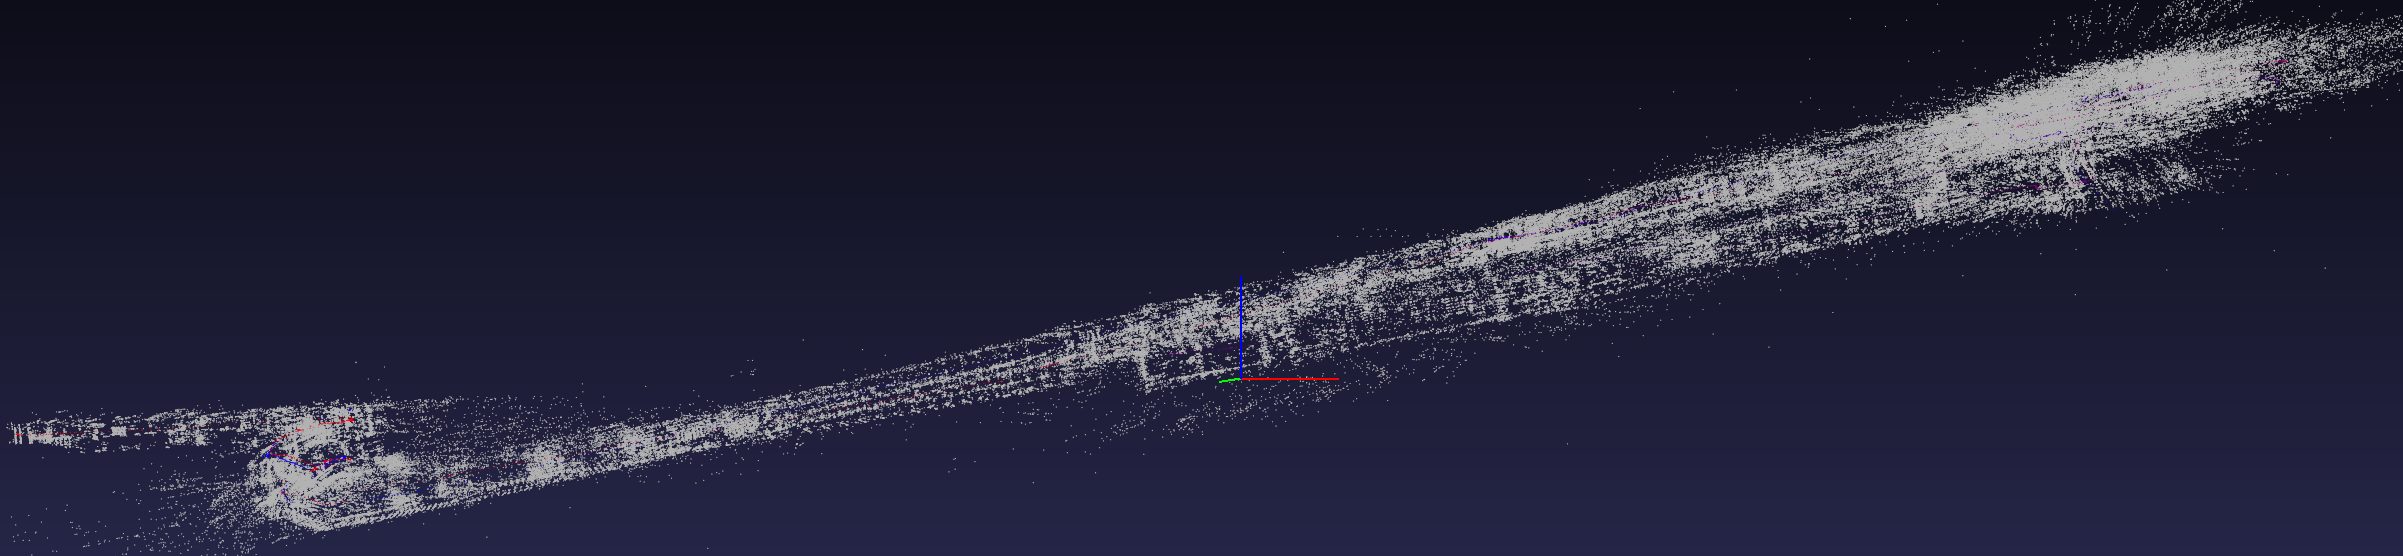
\includegraphics[width=\textwidth]{openvslam_kampusareena_side.png}
    \caption{%
        Side view of the same map as in~\cref{fig:openvslam_kampusareena_top}.
        Drift in the orientation is noticeable in the stairwell.
    }\label{fig:openvslam_kampusareena_side}

    \vspace{1em}

    \begin{subfigure}[t]{.24\textwidth}
        \centering
        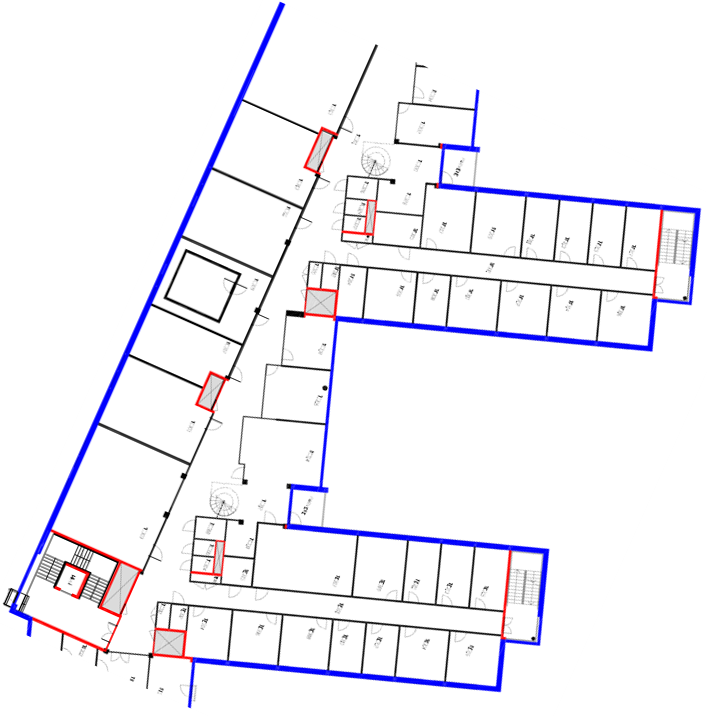
\includegraphics[height=4cm]{corridor_rot.png}
        \caption{Floor plan.}\label{fig:openvslam_tietotalo_corridor}
    \end{subfigure}%
    \begin{subfigure}[t]{.24\textwidth}
        \centering
        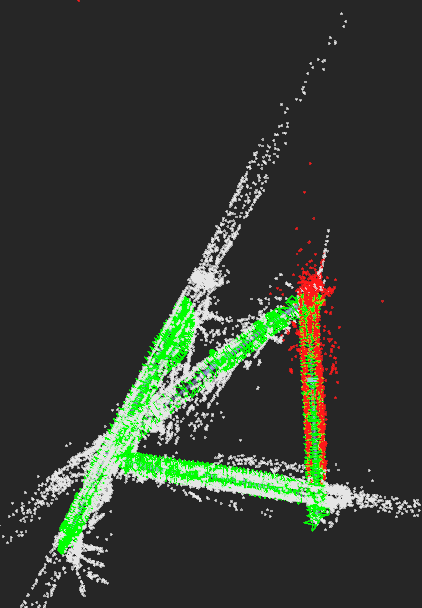
\includegraphics[height=4cm]{openvslam_tietotalo_with_lc.png}
        \caption{A session, loop closures enabled.}\label{fig:openvslam_tietotalo_with_lc}
    \end{subfigure}%
    \begin{subfigure}[t]{.24\textwidth}
        \centering
        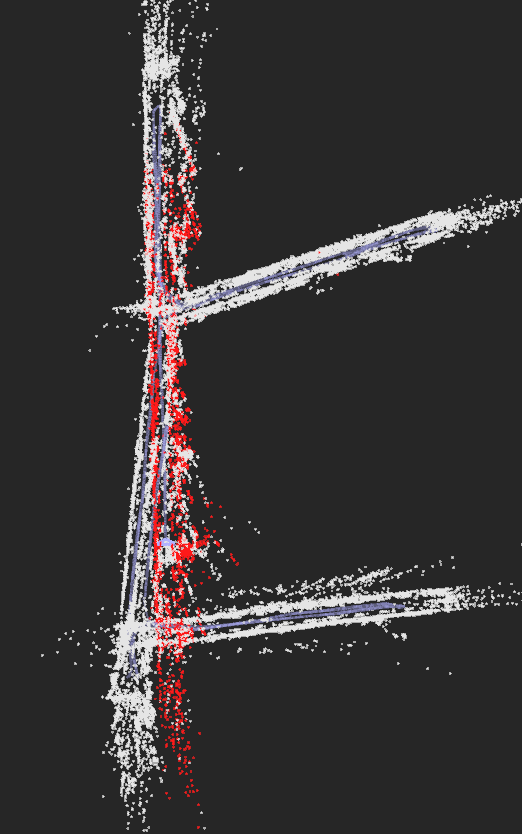
\includegraphics[height=4cm]{openvslam_tietotalo_without_lc}
        \caption{A different session, loop closures disabled.}\label{fig:openvslam_tietotalo_without_lc}
    \end{subfigure}%
    \begin{subfigure}[t]{.24\textwidth}
        \centering
        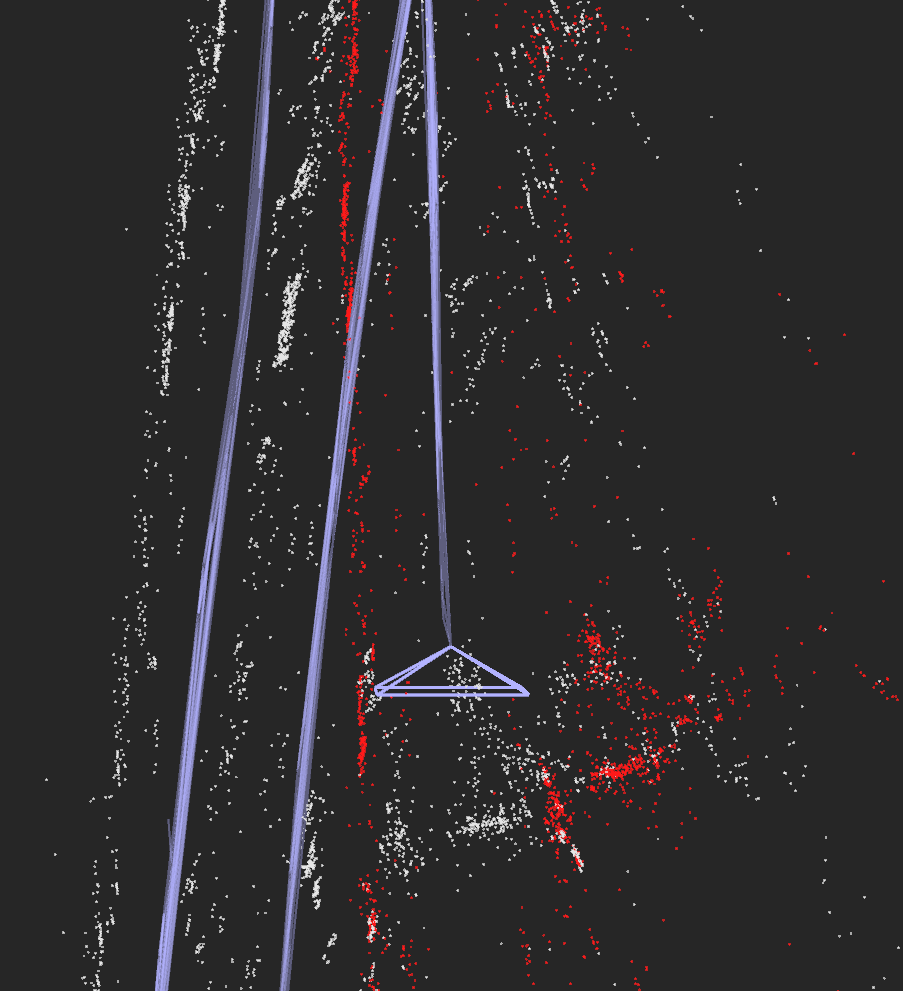
\includegraphics[height=4cm]{openvslam_tietotalo_without_lc_detail}
        \caption{Detail from \cref{fig:openvslam_tietotalo_without_lc}.}\label{fig:openvslam_tietotalo_without_lc_detail}
    \end{subfigure}%

    \caption{%
        Mapping of the same office space as in \cref{fig:rtabmap_lc}, performed
        with OpenVSLAM using as input the rectified stereo pair from the ZED
        camera. Wrong loop closures and drift are the most evident issues.
    }\label{fig:openvslam_lc}
\end{figure}

\begin{figure}[tb]
    \centering

    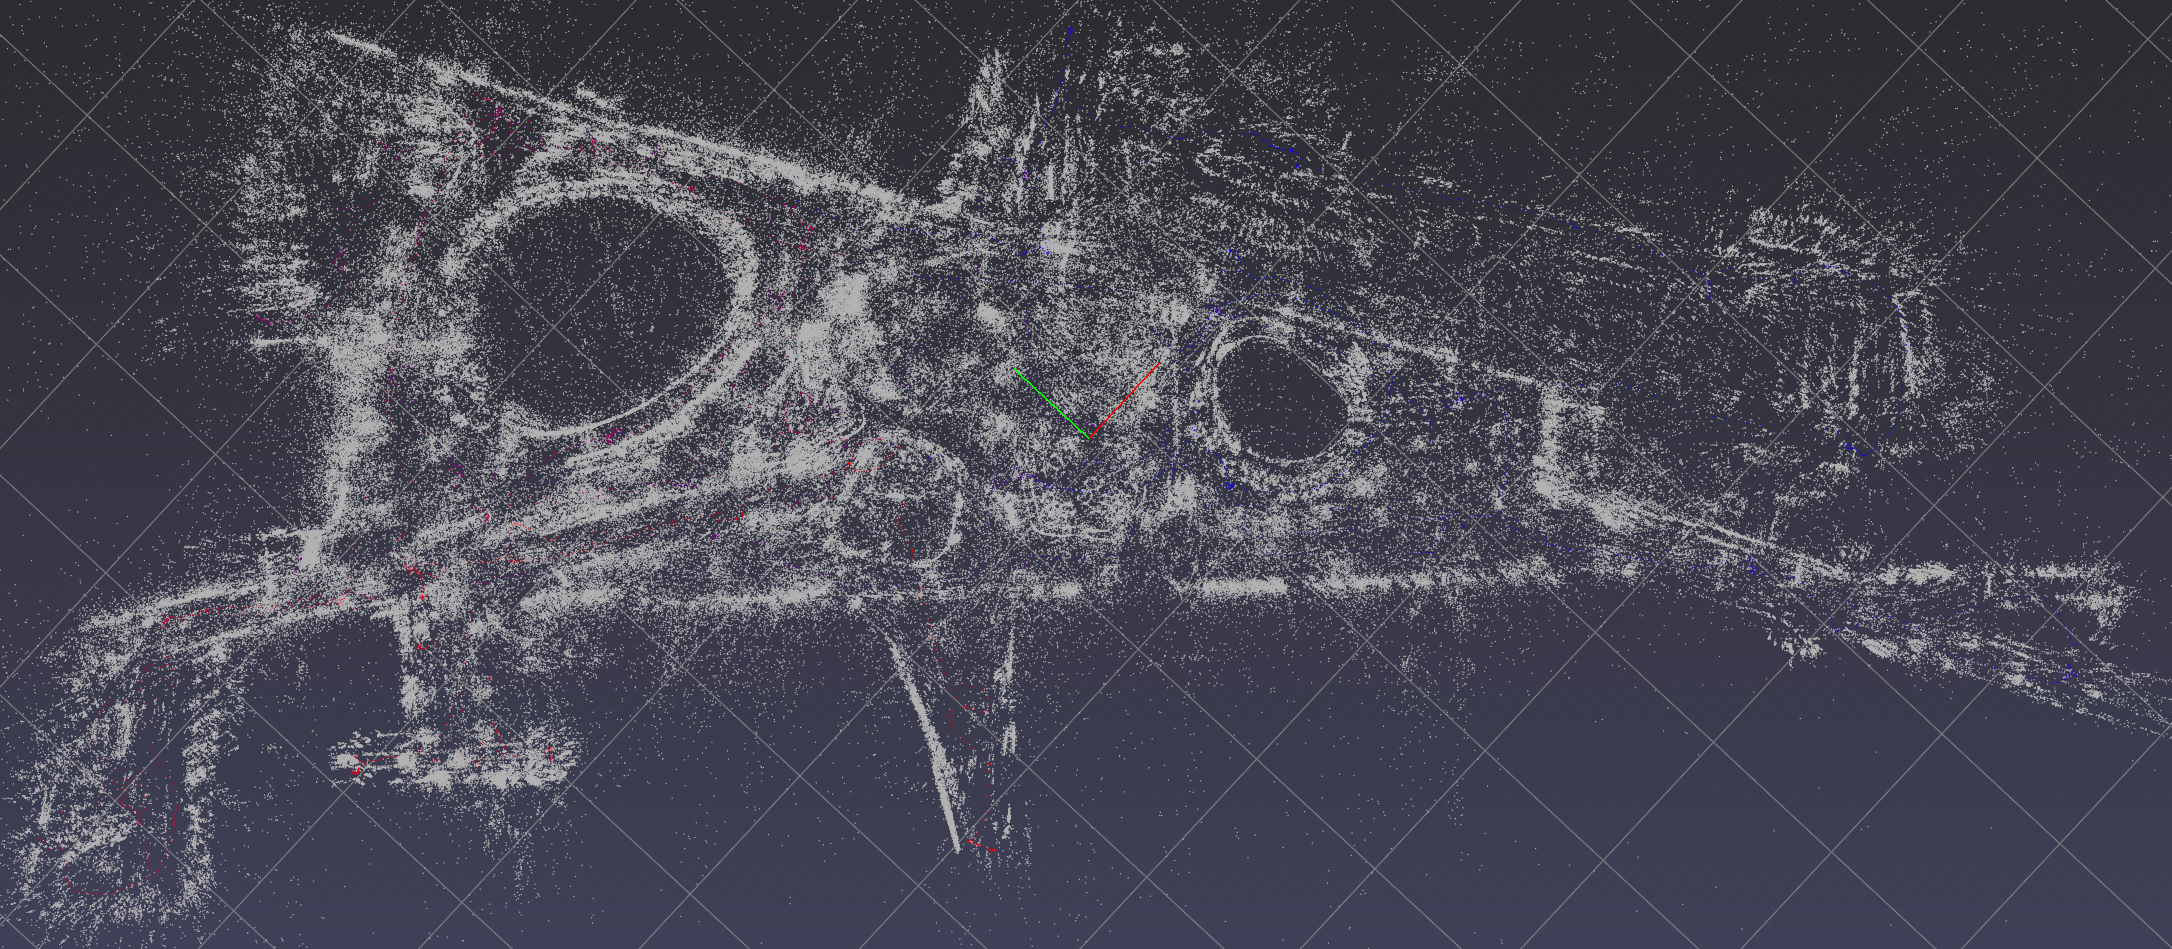
\includegraphics[width=\textwidth]{openvslam_kampusareena_map_top.png}
    \caption{%
        Map of the first and second floors of Kampusareena (396~723 keypoints),
        generated with OpenVSLAM using as input the rectified stereo pair from
        the ZED camera.
    }\label{fig:openvslam_kampusareena_map_top}

    \vspace{1em}

    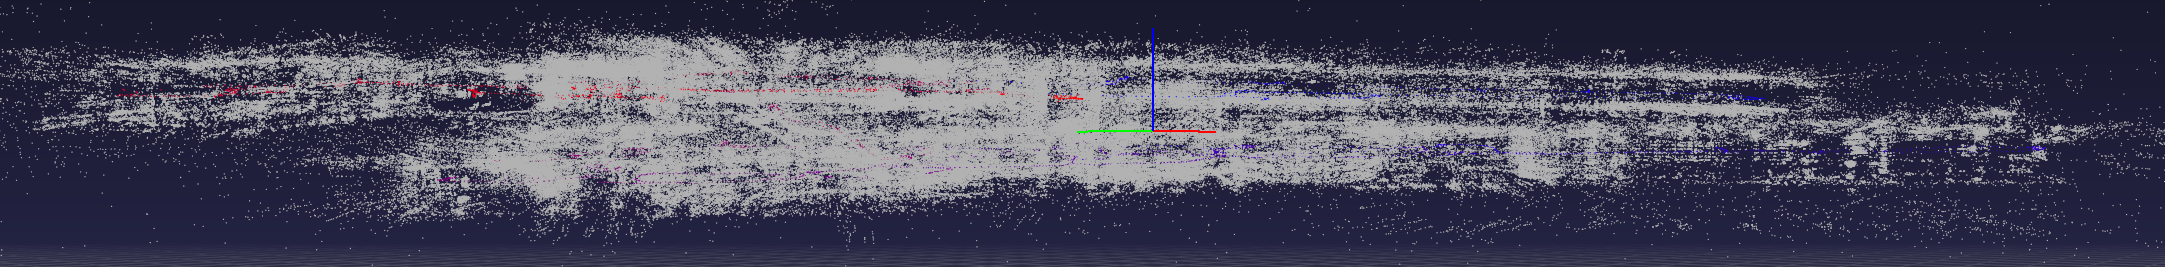
\includegraphics[width=\textwidth]{openvslam_kampusareena_map_side.png}
    \caption{%
        Side view of the same map as in~\cref{fig:openvslam_kampusareena_map_top}.
    }\label{fig:openvslam_kampusareena_map_side}
\end{figure}

\begin{figure}[tb]
    \centering
    \begin{subfigure}[t]{.49\textwidth}
        \centering
        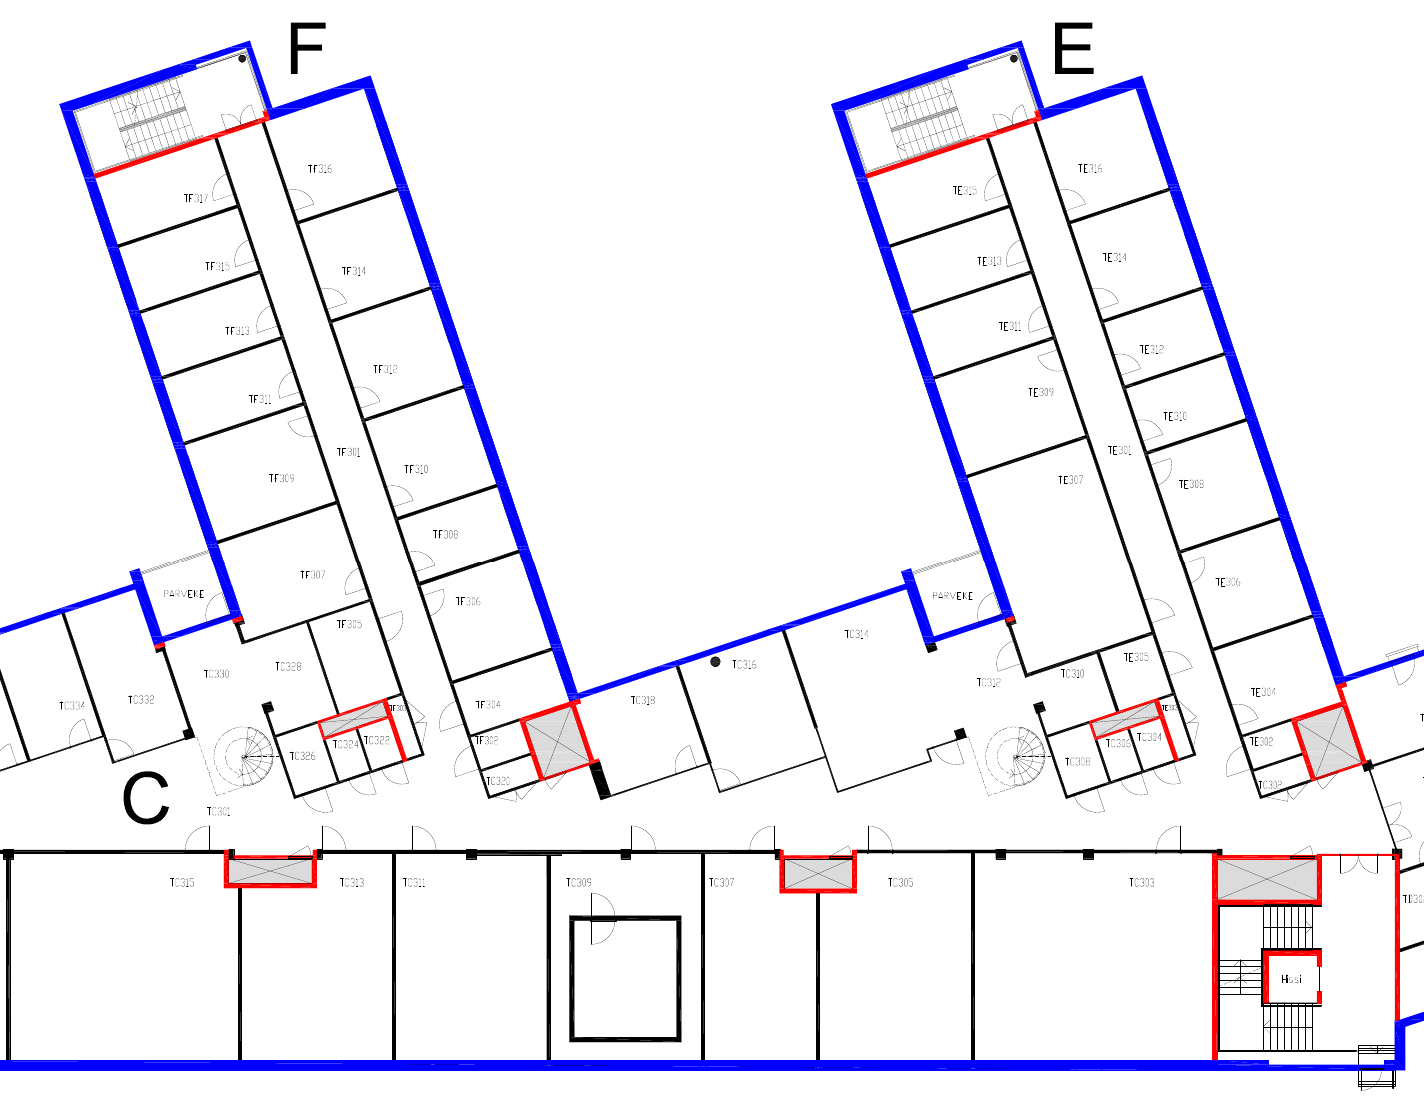
\includegraphics[height=6cm]{corridor.png}
        \caption{Floor plan.}\label{fig:kimera_corridor}
    \end{subfigure}%
    \begin{subfigure}[t]{.49\textwidth}
        \centering
        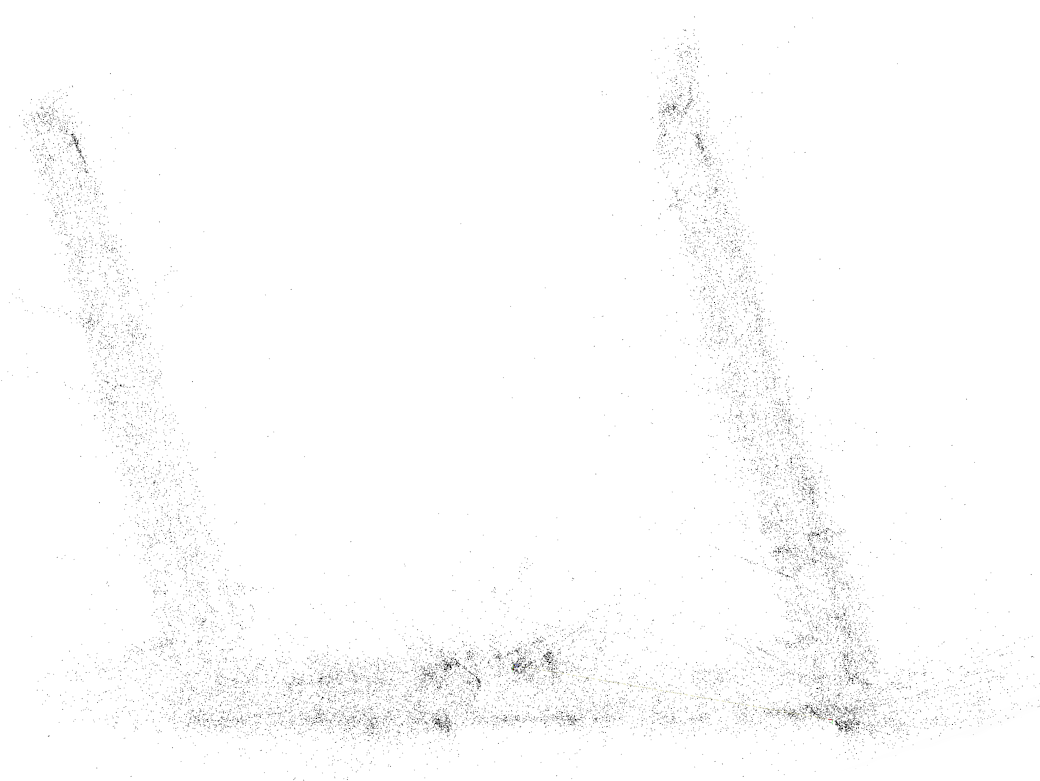
\includegraphics[height=6cm]{kimera_result.png}
        \caption{%
            Map keypoints generated by Kimera-VIO.
        }\label{fig:kimera_result}
    \end{subfigure}%
    \caption{Map generated with Kimera-VIO.}\label{fig:kimera}
\end{figure}

\FloatBarrier{}

\bibliography{bibliography}

\end{document}
